\chapter{Learning coupled dictionaries}
\label{chap_dictionarylearning} 
This chapter describes an alternative approach to learn the relation between large and small scales of turbulence based on \textit{dictionary learning} methods. The approach finds coupled dictionaries to represent the low and high resolution turbulent fields and to reconstruct the missing small-scale information. This method has been applied successfully in image processing, and remains a very active research subject. It potentially outperforms regression models, which are sometimes too simplistic to represent the underlying phenomenon in turbulence. Indeed learned dictionaries could encode part of the physics of the flow. 

This chapter is organized as follows. First, different data representations are discussed, from predefined bases such as Fourier or wavelets to learned bases such as principal component analysis (PCA). Second, dictionary learning, a generalization of PCA, is discussed for the first time as a representation for turbulent fields. This section reviews also two algorithms to learn the dictionaries. Third, different approaches to learn coupled dictionaries of low and high resolution fields are presented. Last, the approach is tested on the DNS database of an isotropic turbulence presented in section \ref{sec:data_isotropic}. 

\section{From bases to dictionaries}
This section briefly reviews conventional representations of turbulent signals. Given a vector $ \x_t $, the main idea of all representation methods is to find a ``\textit{dictionary}'' $ \dict $, a set of basis functions or the so-called ``\textit{atoms}'' from which $ \x_t $ can be represented via a linear combination. This representation by coefficients $ \adictco_t $ is called a ``\textit{code}''. The representation can be exact:
\begin{equation}
\x_t = \dict \adictco_t
\end{equation}
or approximate:
\begin{equation}
 \x_t = \dict \adictco_t +\n_t
\end{equation}
where $ \n_t $ is an estimation noise term. Seeking the representation of the signal is an optimization problem to estimate the dictionary $ \dict $ and the code $ \adictco_t $. The dictionary can be mathematically predefined or learned from the data. The estimation of the coefficients $ \adictco_t $ can be very simple with very fast algorithms for predefined or orthogonal bases, or more complex with redundant dictionaries. 

\subsection{Predefined dictionaries}
Various types of dictionaries are studied to represent the data. They can be predefined \textit{a priori} such as the well-known Fourier transform, the group of \textit{wavelets} or \textit{curvelets} \citep{mallat1989theory,mallat1999wavelet}. These predefined transforms are easy to compute thanks to fast algorithms. Fourier transform aims at describing the signal via its frequency content by decomposing signals as an infinite series of sines and cosines. This transformation is localized in frequency but not in space/time. The constraint is overcome using wavelet transforms, replacing the sines and cosines by wavelet functions localized both in space/time and frequency. This property permits wavelets to better represent the signal with discontinuities or sharp spikes. In such cases, the representations are much more compact with wavelet functions than sines and cosines. This makes wavelets standard in signal compression, for example JPEG 2000 for images, while Fourier transform is mainly used for spectral analysis.

Representations using predefined bases suffer from some limitations. Fourier transform is limited to spectral analysis due to its localization in frequency. Wavelet transforms overcome this constraint by its carefully designed functions, which permit the localization both in space/time and frequency domain. The aim is to optimize the ``\textit{sparsity}'' of the representation, which is to minimize the number of basis functions to accurately represent the data. However, despite the large family of wavelets, all kinds of signals cannot be represented with high level of sparsity. Analogously for turbulence data, different flows or a single flow at various positions with respect to a wall can have significantly different physics, leading to signals with completely different properties.

\subsection{Adaptive dictionaries}
To further optimizing the representation, it is more appealing to learn dictionaries adaptively from the data \citep{bengio2013representation}. The first and most common method is the \textit{principal component analysis} (PCA). This approach learns a basis that maximizes the variance of the projected values. This is interesting for turbulence studies, since large scales of higher variances are of interest. This representation imposes orthogonal bases, which implies that the number of atoms is limited by the dimension of the input vectors. PCA is potentially subject to certain limitations due to this constraint. This chapter discusses the generalized version of PCA, which permits to learn a ``\textit{redundant}'' dictionary. The method is called \textit{dictionary learning}, which is widely used and remains an active research topic in image processing. It will be discussed further in this section before applying to the problem of turbulent field reconstruction. 

Adaptive dictionaries are useful in many applications \citep{tovsic2011dictionary}. The first one is \textit{dimension reduction} \citep{burges2010dimension}, which is useful to build models or visualize large amount of data. For modeling, high dimensional input variables potentially causes the problem of high variance as discussed in chapter \ref{chap_linearregression}, or intractable computation complexity. For visualization, it is a real constraint since the maximum number of dimensions one can observe and analyze is probably no more than three. The core idea is to project data onto a set of atoms in a dictionary. This projection is lossy, meaning that a certain amount of less informative variance is discarded. Another important application is to solve inverse problems such as super-resolution or denoising. These problems are very ill-posed and can not be solved directly by least-squares methods. A good representation of the data can play the role as a regularization term, making the problem easier to solve. The choice of a dictionary defines the space in which we search for solutions.

\section{Proper Orthogonal Decomposition (POD) as a representation of turbulent fields}
PCA \citep{jolliffe2002principal}, known also as \textit{Karhunen–Loève} transform, is commonly used in many fields of signal and image processing. It was first introduced in turbulence studies by \citet{lumley1967} under the name ``\textit{proper orthogonal decomposition}'' (POD). It is then used as a standard approach for dimensionality reduction, which is largely beneficial in large scales reconstruction, flow control and coherent structure studies. PCA decomposes a sequence of snapshots into a dictionary $ \dict $ to represent spatial structures, and a coefficient matrix $ \dictco $, to capture temporal dynamics. The works on coherent structures and flow information extraction focus on the dictionary $ \dict $ \citep{bonnet1994stochastic, gordeyev2000coherent}. Each atom $ \adict_i $, as ranked by its variance (an equivalent measure of the kinetic energy), represents the most energetic structures of the flow. Flow control and modeling works focus more on the use of projection coefficients $ \dictco $. After learning the fixed dictionary $ \dict $, independent of time, from given training fields, the temporal dynamics of the flow is presented in the projection coefficients $ \dictco $ only. The efforts to model and control the flow are reduced tremendously by considering only several coefficients of high-variance atoms. This property is beneficial for reduced-order modeling works in flow control and reconstruction of large-scale velocity fields \citep{ravindran2000reduced, ly2001modeling, taylor2004towards}.

To derive POD or PCA, let first denote a data matrix $ \X $ of size $ \dimsh \times \dimtl $ containing a sequence of $ \dimsh- $dimensional input vectors $ \x_t, t=1,2,...,\dimtl $,
\begin{equation}
\X \mydef \begin{bmatrix} \x_1, \x_2, ..., \x_\dimtl \end{bmatrix},
\end{equation} 
assumed centered \textit{a priori}:
\begin{equation}
\sum\limits_{t=1}^{\dimtl}\x_t = \mybold{0}
\end{equation}
From $ \X $, a dictionary $ \dict $ of size $ \dimsh \times \dimsh $ is estimated, which contains $ \dimsh $ atoms $ \adict_i \in \R ^\dimsh, i=1,2,...,\dimsh  $. The objective is to project $ \x_t $ onto a reduced-order subspace of dimension $ \dimtrunc \leq \dimsh $ while maximizing the amount of variance. This idea, when applying to turbulent fields where variance represents the kinetic energy, is interpreted as determining the most energetic structures among a sequence of snapshots. 

The first step is to find the most dominant basis function $ \adict_1  \in \R^\dimsh$, assuming $ \normtwo{\adict_1} = 1 $. Each input vector is projected onto this direction as $ \adict_1^\mytrans \x_t $. The variance of this projection is:
\begin{equation}
s_1 = \frac{1}{\dimtl} \sum\limits_{t=1}^{\dimtl}\left( \adict_1^\mytrans \x_t\right)^2 =  \adict_1^\mytrans \Sigma \adict_1
\end{equation}
where $ \Sigma  $ is the covariance matrix:
\begin{equation}
\Sigma = \frac{1}{\dimtl} X X^\mytrans
\end{equation}
The aim now is to find  $ \adict_1 $ such that $ s_1 $ is maximum, with the constraint that $ \normtwo{\adict_1} = 1$:
\begin{equation}
\adict_1 = \argmax_{\adict_1}{ \left\lbrace \adict_1^\mytrans \Sigma \adict_1 \right\rbrace } \:\:\:\:\:\: s.t \:\:\:\:\:\: \normtwo{\adict_1} = 1
\end{equation}
This optimization problem can be rewritten in an unconstrained manner by introducing a Lagrange multiplier $ \lambda_1 $:
\begin{equation}
\adict_1 = \argmax_{\adict_1}{ \left\lbrace \adict_1^\mytrans \Sigma \adict_1 + \lambda_1 \left(1-\adict_1^\mytrans \adict_1\right) \right\rbrace } 
\end{equation}
Setting the derivative with respect to $ \adict_1 $ to zero, one obtains:
\begin{equation}
\Sigma \adict_1 = \lambda_1 \adict_1
\end{equation}
which implies that $ \adict_1 $ is an eigenvector of $ \Sigma $, and $ \lambda_1 $ is the equivalent eigenvalue. Also, multiplying both side with $ \adict_1^\mytrans $, using $ \adict_1^\mytrans\adict_1=1 $, one has:
\begin{equation}
\adict_1^\mytrans \Sigma \adict_1 = \lambda_1
\end{equation}
The above expression implies that $ \lambda_1 $ is the variance of the projection onto $ \adict_1 $. This variance is maximized by selecting the maximum eigenvalue of the covariance matrix $ \Sigma $. This process is repeated to find the second basis of the dictionary $ \adict_2 $ such that it is orthogonal to the first one, i.e. $ \adict_1^{\mytrans}\adict_2=0 $. This is identical to find the second eigenvector corresponding to the second largest eigenvalue $ \lambda_2 $. The procedure of seeking all $ \dimsh $ bases is identical to eigenvalue decomposition and SVD of the covariance matrix $ \Sigma $. Sorting $ \dimsh $ eigenvalues in a descending order as $ \lambda_1 \geq \lambda_2 \geq ... \geq \lambda_\dimsh \geq 0 $, one obtains the dictionary, or codebook, learned from the training samples $ \X $ by putting the equivalent eigenvectors together as $ \dict \mydef \left[ \adict_1, \adict_2, ..., \adict_\dimsh \right] $. The projection matrix $ \dictco $ is found such that:
\begin{equation}
\X = \dict \dictco
\end{equation}


\section{Dictionary learning as a new representation}
Due to the orthogonality and variance maximization properties, PCA gains its success in many problems such as dimensionality reduction, low-order modeling and lossy compression. However, in solving different inverse problems, PCA is subject to several limitations. The number of atoms is at most the dimension of input vectors, leading to the ``limited expressiveness'' property \citep{tovsic2011dictionary}. The representation learned by PCA can be efficient for training data, but a good generalization is not guaranteed. It is desirable to ignore the constraint on the number of basis functions and learn a redundant dictionary. Due to the redundancy, the sparsity constraint can be imposed and play the role of the regularization to solve ill-posed inverse problems.

\subsection{Redundant dictionary and sparse representation}
Dictionary learning (DL) ignores the constraint on the number of basis functions, or atoms, permitting to find a \textit{redundant} (or \textit{overcomplete}) dictionary $ \dict \in \R^{\dimsh \times \dimdict} $ to represent the data. $ K $ is the number of atoms, and redundancy means that $ \dimdict $ is potentially larger than $ \dimsh $. These vectors are therefore not necessarily orthogonal. The companion of redundancy is sparsity, where the linear transformation matrix $ \dictco $ contains only a few nonzero coefficients. The representation then relies on the duality between redundancy and sparsity, which will be discussed further in this section. With more atoms, the representation using dictionary learning is expected to be more adaptive to the signal and to better represent new data. This is the reason why the approach often gives the state-of-the-art results in most inverse problems in image processing \citep{elad2010on,yang2010image}.

The problem of representing data $ \X $ using the redundant dictionary $ \dict $ and sparse coefficients $ \dictco $ includes two alternating optimization problems. The first one is to estimate the projection coefficients $ \dictco $. PCA, with the orthogonality among atoms, simply estimates $ \dictco $ by dot products. Dictionaries, which are not necessarily orthogonal, can have more atoms than the dimension ($ \dimdict > \dimsh $). There are potentially many matrices $ \dictco $ such that $ \X = \dict \dictco $. The sparsity constraint, meaning that $ \dictco $ has a minimal number of nonzero coefficients, is imposed to make the solution unique. The representation of $ \X $ becomes approximate, i.e. $ \X \approx \dict \dictco $. Finding $ \dictco $ becomes an optimization problem of the form:
\begin{equation}
\dictco = \argmin_{\dictco}{\normp{\dictco}} \quad s.t. \quad \X = \dict \dictco
\end{equation}
or re-arranged in the form of a regularized cost function as in chapter \ref{chap_linearregression}:
\begin{equation}
\dictco = \argmin_{\dictco}{\normtwo{\X - \dict \dictco} + \lambda \normp{\dictco}}
\end{equation}
The common \textit{$ \ell^p $ norm} $ \normp{.} $ is with $ 0 \leq p \leq 1 $. Solving the problem with the $ \ell^0 $ norm, i.e. counting the number of nonzero coefficients, leads to orthogonal matching pursuit (OMP) \citep{tropp2007signal}, while solving with the $ \ell^1 $ norm, summing the absolute values of the coefficients, leads to LASSO as discussed in chapter \ref{chap_linearregression}. Least Angle Regression (LARS) \citep{efron2004least} is sometimes used as another efficient algorithm to solve $ \ell^1 $ penalty problems and gives results very similar to LASSO. These regularizations help selecting a limited number of atoms that best approximate the input $ \X $. The second problem is the choice of the dictionary, which is solved by efficient algorithms discussed in the next section.

\subsection{Dictionary learning methods}
Many algorithms have been proposed to learn the dictionary from data, starting with gradient descend method \citep{olshausen1996emergence}, then K-SVD \citep{aharon2006ksvd}, feature-sign approach \citep{lee2006efficient} and online dictionary learning \citep{mairal2010online}. This section reviews some of those that are used later in this chapter. 

\subsubsection{Alternate optimization}
Dictionary learning is an alternate optimization problem to search the redundant dictionary $ \dict $ and the sparse matrix $ \dictco $. The approach has started by using a gradient descent approach \citep{olshausen1996emergence}. It has recently gained popularity thanks to the progress in solving regularized optimization problems with $ \ell^p $ penalty \citep{tibshirani1996regression, donoho2003optimally, efron2004least, donoho2012sparse}. One of the first efficient dictionary learning approach is the \textit{method of optimal directions} (MOP) \citep{engan1999method} where $ \dict $ and $ \dictco $ are estimated by solving:
\begin{equation}
(\dict, \dictco) = \argmin_{\dict, \dictco} \normtwo{\X - \dict \dictco} \subjectto \normzero{\adictco_t} < \dimtrunc \quad \forall t
\end{equation}
$ \dimtrunc $ is the sparsity constraint- the maximum number of nonzero coefficients. This optimization problem is  combinatorial and highly non-convex. The search for a local minimum is done by alternating two steps. With a fixed dictionary $ \dict $, the \textit{sparse coding} step finds the representation of the input vectors by solving:
\begin{equation}
\dictco = \argmin_{\dictco} \left\lbrace \normtwo{\X - \dict\dictco} + \lambda \normp{\dictco}\right\rbrace
\end{equation}
This step uses OMP for $ \ell^0 $ penalty and LASSO or LARS for $ \ell^1 $ penalty. The \textit{dictionary update} step re-estimates $ \dict $ with fixed $ \dictco $ via the Moore-Penrose pseudo-inverse:
\begin{equation}
\dict = \X \dictco^\mypseudo = \X \dictco^\mytrans (\dictco \dictco^\mytrans)^{-1}
\end{equation}
This scheme converges rapidly after some iterations, but requires complex matrix inversion, which is not efficient in most cases \citep{aharon2006ksvd}. 
\subsubsection{K-SVD}
The \textit{K-SVD} algorithm was proposed later by \citet{aharon2006ksvd} and rapidly gained its popularity. The \textit{dictionary update} is done by a block-relaxation approach. Instead of inversing the matrix, the algorithm updates each atom in an efficient way by generalizing the \textit{k-means} clustering method \citep{bishop2006pattern}. The $ k- $th atom is estimated by minimizing a quadratic error:
\begin{equation}
	\left\lbrace \adict_k, \adictco_k \right\rbrace = \argmin_{\adict_k, \adictco_k} \normtwo{E_k \: - \: \adict_k \adictco_k^\mytrans}
\end{equation} 
where $  E_k $ is defined as the residual matrix:
\begin{equation}
E_k \mydef \X_k \: - \: \sum_{j\neq k} \left(\adict_j \adictco_j^\mytrans \: - \: \adict_k \adictco_k^\mytrans\right)
\end{equation}
where $ \X_k $ gathers examples $ \x_t $ using $ \adict_k $ in their representation. The update of both $ \adict_k $ and $ \adictco_k $ is done simultaneously via a rank-1 approximation, i.e. considering only the first eigenvector of $ E_k $ after performing a SVD.

\subsubsection{Online dictionary learning (ODL)}
K-SVD algorithm has certain constraints, mainly with a potential local minimum while iteratively learning the dictionary \citep{rubinstein2010dictionaries}. The algorithm is also limited to small numbers of samples due to its computational cost. Online dictionary learning (ODL) has been proposed by \citet{mairal2010online} to learn $ \dict $ from massive datasets. The use of stochastic gradient descent to update the dictionary for each example (or a group of them), and LARS algorithm for sparse coding, permits the learning over millions of samples. Algorithm \ref{algo_ODL} summarizes this approach.

\begin{algorithm}[t]
\caption{Online dictionary learning algorithm by  \citet{mairal2010online}} \label{algo_ODL}
\begin{algorithmic}[1]
	\State Input: 
	\begin{itemize}
		\item a set of $ \mathcal{S}(\x) $ of $\dimtl $ input variable $ \x_t \in \R^\dimsh$;
		\item $\lambda \in \R $ : regularization parameter ($ \lambda \geq 0 $)
		\item $ \dict_0 \in \R^{\dimsh \times K}$: initial dictionary
	\end{itemize}
	\State $ \mathbf{G}_0 \gets  0$, $ \mathbf{H}_0 \gets 0 $
	\For {$ t = 1, 2, ..., \dimtl$}
		\State Draw $ \x_t $ from $\mathcal{S}(\x)$
		\State Sparse coding:
		\begin{equation}
			\adictco_t = \argmin_{\adictco \in \R^K} \left\lbrace \x_t - \dict_{t-1}\adictco +\lambda \normone{\adictco}\right\rbrace
		\end{equation}
		\State $ \mathbf{G}_t \gets \mathbf{G}_{t-1}+\adictco_t \adictco_t^\mytrans$
		\State $ \mathbf{H}_t \gets \mathbf{H}_{t-1}+\adictco_t \x_t^\mytrans$
		\State Update $ \dict_t $:
		\begin{equation}
			\begin{split}
			\dict_t = & \argmin_{\dict \in \mathcal{C}} \left\lbrace \frac{1}{t} \sum\limits_{i=1}^{t}\frac{1}{2} \normtwo{\x_i - \dict\adictco_i} + \lambda \normone{\adictco_i} \right\rbrace \\
			=& \argmin_{\dict \in \mathcal{C}} \left\lbrace \frac{1}{t} \sum\limits_{i=1}^{t}\frac{1}{2} \mytrace{\dict^\mytrans\dict \mathbf{G}_t} - \mytrace{\dict^\mytrans \mathbf{H}_t} \right\rbrace
			\end{split}
		\end{equation}
	\EndFor
	\State Return $ \dict_\dimtl $
\end{algorithmic}
\end{algorithm}

\section{Learning coupled dictionaries}
\label{joint_learning}
In this section, DL is used to solve the problem of reconstructing HR fields from LR ones. The approach is inspired by the \textit{single image super-resolution} application \citep{yang2010image,yang2012coupled,zeyde2012single}, i.e. estimating HR images with finer details from LR ones. The approach jointly learns coupled dictionaries at LR and HR from given training samples. These dictionaries are forced to represent the data using the same coefficients. In the prediction phase, the projection coefficients are estimated from the LR images and then combined with the learned HR dictionary to reconstruct the HR images. 

\subsection{Patch-based approach}
\label{subsec:patch_based_estimation}
\begin{figure}
\centering
	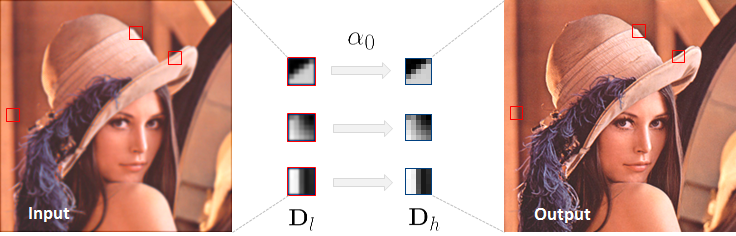
\includegraphics[width=0.9\textwidth]{./images/DL/ScSR.png}
	\caption{\label{fig:ScSR} An example of single image super-resolution using coupled dictionary learning and patch-wise approach. Photo credit: \citet{yang2010image}.}
\end{figure}

DL requires a sparse coding step, i.e. solving the $ l^1 $-penalty optimization problem. The computation complexity is $ \mathcal{O}(\dimsh^3+\dimtl\dimsh^2) $ \citep{efron2004least}, where $ \dimsh $ is the dimension of the fields and $ \dimtl $ is the number of samples. Since $ \dimsh \gg \dimtl$ in most cases, the complexity is $ \mathcal{O}(\dimsh^3) $, which is a very heavy procedure. The computation is therefore intractable with the whole field. To overcome this difficulty, the ``\textit{patch-wise}'' approach uses small patches instead of the whole fields. These patches are extracted from the original fields at all positions by moving pixel-by-pixel in both horizontal and vertical directions. Let $ \dimptl $ be the total number of patches, and $ \dimpsh $ be their dimension ($\dimptl \gg \dimpsh $), the computation complexity becomes $ \mathcal{O}(\dimptl\dimpsh^2) $, which is tractable when $ \dimpsh $ is small. In the reconstruction phase, since one pixel belongs to several intersecting patches, the estimated field is reconstructed by aggregating all possible estimates of each pixel after putting them back into the whole scene.

The path-wise approach comes with several advantages. First, it localizes the information. A shared dictionary can be learned to represent all type of images with different contents. Second, it reduces tremendously the computation. Standard images are of dimension few millions, while typical patch sizes are around $ 8 \times 8 $, which is a few orders of magnitude smaller. Last, since the learning is on small patches, the number of samples required for the algorithm to converge is much smaller. From a single image, millions of small patches can be extracted for learning. Working with the original image, the number of training samples is necessary at least one order of magnitude higher than its dimension, which is already millions of pixels. 

To formulate the patch-based approach, let $ \z_t \in \R^{\dimsh} $ be a snapshot of a high-resolution field as a column vector. The operator $ \extracthigh{k}:\R^{\dimsh} \mapsto \R^{\dimpsh} $ is to extract the 2D patch and put them in a lexicographical order to form a column vector $ \patchhigh{k} \mydef \extracthigh{k} \z_t \in \R^\dimpsh $, where $ \dimpsh $ is the size of 2D patches $ \patchhigh{k} $. If the overlapping is such that all patches are translated pixel-by-pixel, the total number of patches is $ \left( \sqrt{\dimsh} - \sqrt{\dimpsh} + 1 \right)^2 $. The reconstruction of the whole image is done as:
\begin{equation}
\hat{\z}_t= \left[ \sum\limits_{k} \left(\extracthigh{k}\right)^{\mytrans}\extracthigh{k}\right]^{-1}\sum\limits_{k} \left(\extracthigh{k}\right)^{\mytrans}\hat{\mybold{p}}_h^k
\end{equation}
where $ \hat{\mybold{p}}_h^k $ and $ \hat{\z}_t $ are the estimates of the reference $ \patchhigh{k} $ and $ \z_t $ respectively. The term $ \left(\extracthigh{k}\right)^{\mytrans}: \R^{n} \mapsto \R^{\dimsh}$ puts the equivalent patch into the global 2D scene and zero-pad elsewhere. The term $ \left(\extracthigh{k}\right)^{\mytrans}\extracthigh{k} $ just counts the number of estimates for each pixels. Its inversion plays the role of a normalization factor. In practice, the whole process is done by estimating each pixel as its mean or median of all estimates from all patches that it belongs to. 

\subsection{The approach}
\label{sec:chap3_theapproach}
Let assume that small patches from the field can be represented as a linear combination of several atoms from the learned dictionary. This assumption is the so-called ``\textit{Sparse-Land}'' prior \citep{zeyde2012single}. The idea is to learn coupled dictionaries by imposing that the representation coefficients are the same at low and high resolution. The following section recalls the main ideas. More details can be found in \citet{zeyde2012single}.

Suppose that $ \z_t \in \R^{\dimsh}$ is the true high resolution velocity field. The corresponding low-resolution field $ \y_t \in \R^{\dimsl} $ $(\dimsl < \dimsh) $ is obtained as:
\begin{equation}
\y_t = \Sub_s\LPF_s\z_t + \mybold{v}_t
\label{eq:DL_approach1}
\end{equation}
where $ \mybold{v}_t $ is a random noise, $ \LPF_s $ is an anti-aliasing low-pass filter, and $ \Sub_s $ is a subsampling operator. The presence of $ \LPF_s $ is to avoid the problem of aliasing when subsampling the field. In the case of direct subsampling, this filter is omitted from the above model. The goal is to find a HR estimate $ \hat{\z}_t $ containing both large and small scales. The most naive and simple idea is to interpolate from $ \y $, i.e. $ \hat{\z}_t = \Interp_s\y_t \in \R^{\dimsh}$. However, it will give no access to small-scale information above the cutoff frequency defined by the low-resolution grid. The coupled dictionary approach permits to learn small scales from training data and uses it for the reconstruction. 

DL uses the patch-based approach, where the couples of LR and HR patches are extracted from the LR and HR fields respectively. Let $ \patchhigh{k} = \mathcal{R}_h^k \z_t \in \R^\dimpsh $ be the $ k-${th} HR patch. By assuming the Sparse-Land model for high and low resolution training fields, each patch can be estimated as a linear combination of atoms in a dictionary:
\begin{equation}
\patchhigh{k} = \dict_h \adictco^k + \mybold{\epsilon}^k
\label{eq:DL_approach2}
\end{equation} 
where $ \dict_h  \in  \R^{\dimpsh \times K}$ is the HR dictionary, $ \adictco^k \in \R^K$ is the coefficient vector and $ \mybold{\epsilon}^k $ is the reconstruction error. The dictionary is redundant ($ K > \dimpsh $) and the coefficients are sparse ($ \Arrowvert \adictco^k \Arrowvert_0 < \dimtrunc $), with the sparsity constraint $ \dimtrunc \ll K $. The corresponding LR patch $ \patchlow{k} \in \R^\dimpsl $ is: 
\begin{equation}
	\patchlow{k} = \extractlow{k} \y_t = \extractlow{k} \Sub_s\LPF_s\z_t + \extractlow{k}\mybold{v}_t
\label{eq:DL_approach3}
\end{equation}	
$ \extractlow{k} $ is just an extraction operator, and $ \Sub_s\LPF_s $ is a transformation operator going from HR to LR fields. Since $ \Sub_s $ and $ \LPF_s $ are spatially independent operators, there exit local $ \Sub_s^{loc} $ and $ \LPF_s^{loc} $ that transform HR to LR patches:
\begin{equation}
	\patchlow{k} =  \Sub_s^{loc}\LPF_s^{loc}\patchhigh{k} + \mybold{v}_\ell^k
	\label{eq:DL_approach4}
\end{equation}  
where $ \mybold{v}_\ell^k $ is a random noise of the same dimension as the LR patches. From equations \ref{eq:DL_approach2} and \ref{eq:DL_approach4}, one can write:
\begin{equation}
\begin{split}
	\patchlow{k} &= \Sub_s^{loc}\LPF_s^{loc}\dicthigh \adictco^k + \Sub_s^{loc}\LPF_s^{loc}\mybold{\epsilon}^k + \mybold{v}_\ell^k \\
				 &= \Sub_s^{loc}\LPF_s^{loc}\dicthigh \adictco^k + \tilde{\mybold{v}}_\ell^k
\end{split}
\label{eq:DL_approach5}	
\end{equation}
where $ \tilde{\mybold{v}}_\ell^k \mydef \Sub_s^{loc}\LPF_s^{loc}\mybold{\epsilon}^k + \mybold{v}_\ell^k$ is also a random noise term. Denoting $ \dictlow \mydef \Sub_s^{loc}\LPF_s^{loc}\dicthigh  $, the above equation illustrates that there exists also a Sparse-Land model for LR patches. These models for LR and HR patches also share the same sparse coefficient $ \adictco^k $. The LR dictionary is also a downsampled version of the HR one.

\subsection{Joint learning methods}
\label{sec:joint_learning_methods}
In practice, $ \Sub_s\LPF_s $ or $ \Sub_s^{loc}\LPF_s^{loc} $ are usually not given. \citet{yang2010image} has addressed this problem by proposing the approach to jointly learn coupled dictionaries. \citet{zeyde2012single} follow the main idea with some modifications. All approaches contains two main steps: \textit{learning phase} and \textit{reconstruction phase}. The learning phase can be done \textit{offline}, i.e. training \textit{a priori} from the data. With learned dictionaries, the reconstruction phase can be \textit{online}.

Given the training HR velocity fields $ \z_t \in \R^{\dimsh} $, corresponding LR fields are virtually extracted as $ \y_t=\Sub_s\LPF_s\z_t \in \R^{\dimsl}$. Couples of LR and HR patches $ \left\lbrace  \patchlow{k},\patchhigh{k}  \right\rbrace $ are extracted from the training fields as $ \patchlow{k}= \extractlow{k} \y_t\in  \R^\dimpsl $ and $ \patchhigh{k}= \extracthigh{k} \z_t\in  \R^\dimpsh $, where $ \dimpsl $ and $ \dimpsh $ are the size of LR and HR patches respectively, and $ \dimpsh/\dimpsl = \dimsh / \dimsl $. Let $ \mathbf{P}_\ell $ and $ \mathbf{P}_h $ denote matrices of all LR and HR patches:
\begin{equation}
	\begin{split}
		\mathbf{P}_\ell&=\left[\patchlow{1} \:\: \patchlow{2} \:\: ... \:\: \patchlow{\dimptl}\right]_{\dimpsl \times \dimptl} \\
		\mathbf{P}_h&=\left[\mybold{p}_h^1 \:\: \mybold{p}_h^2 \:\: ... \:\: \mybold{p}_h^{\dimptl}\right]_{\dimpsh \times \dimptl}
	\end{split}
	\label{eq:jointlearning1}
\end{equation}
where $ \dimptl $ is the total number of patches, and $ \dimptl = \left(\sqrt{\dimsl} - \sqrt{\dimpsl} + 1\right)^2 \times \dimtl$ at most, where $ \dimtl $ is the number of training planes. The LR patches are collected by one-pixel overlapping, while HR ones are obtained by overlapping $ \dimpsh/\dimpsl $ pixels to ensure the same number of LR and HR patches. Coupled dictionaries $ \left\lbrace \dicthigh ,\dictlow  \right\rbrace $ are learned from the coupled training patches $ \left\lbrace \mathbf{P}_h ,\mathbf{P}_\ell  \right\rbrace $ imposing to share the same sparse representation:
\begin{equation}
\begin{cases}
	\mathbf{P}_h \approx \dicthigh \dictco\\
	\mathbf{P}_\ell \approx \dictlow \dictco\\
\end{cases}
\end{equation}            
The first learning approach is proposed by \cite{yang2010image}, which aims at solving an optimization problem:
\begin{equation}
\left\lbrace \dicthigh ,\dictlow, \dictco  \right\rbrace = \argmin_{\dicthigh ,\dictlow ,A} \left\lbrace \frac{1}{\dimpsh} \Vert \mathbf{P}_h-\dicthigh \dictco\Vert^2_2 + \frac{1}{\dimpsl} \Vert \mathbf{P}_\ell-\dictlow \dictco\Vert^2_2 + \lambda_1 \left( \frac{1}{\dimpsh}+\frac{1}{\dimpsl} \right) \Vert \dictco \Vert_1 \right\rbrace
\label{eq:jointlearning2}
\end{equation}
$ \dictco $ is the shared sparse coefficients, which ensures a compromise between small reconstruction errors of patches and sparsity constraint. The two normalization terms $ 1/\dimpsl  $ and $ 1/\dimpsh $ are to balance the two mean-square error terms. The above cost function can be re-written as:
\begin{equation}
\dict = \argmin_{\dict,\dictco} \left\lbrace \Vert \mathbf{P}-\dict \dictco\Vert^2_2 + \lambda_1 \Vert \dictco \Vert_1 \right \rbrace
\label{eq:jointlearning3}
\end{equation}
where
\begin{equation}
\mathbf{P}= \begin{bmatrix} \frac{1}{\sqrt{\dimpsh}}\mathbf{P}_h \\ \frac{1}{\sqrt{\dimpsl}}\mathbf{P}_\ell \end{bmatrix}, \:\: \dict= \begin{bmatrix} \frac{1}{\sqrt{\dimpsh}}\dicthigh  \\ \frac{1}{\sqrt{\dimpsl}}\dictlow  \end{bmatrix}
\label{eq:jointlearning4}
\end{equation}
This problem can be solved using the standard DL algorithms.

The second approach is proposed by \citet{zeyde2012single}, which contains a direct model to estimate the HR dictionary. The LR dictionary is first learned from LR patches:
\begin{equation}
\left\lbrace \dictlow ,\dictco \right\rbrace =\argmin_{\dictlow, \dictco}  \left\lbrace \normtwo{\mathbf{P}_\ell-\dictlow \dictco} + \lambda_1\Vert \dictco \Vert_1 \right \rbrace
\label{eq:jointlearning5}
\end{equation}
Assuming that the representation of HR patches $ \mathbf{P}_h $ via the HR dictionary $ \dicthigh  $ will share the same sparse code $ \dictco $, HR dictionary is estimated as:
\begin{equation}
\dicthigh  = \argmin_{\dicthigh } \left\lbrace \Vert \mathbf{P}_h-\dicthigh \dictco\Vert^2_2  \right \rbrace
\label{eq:jointlearning6}
\end{equation}
for which the solution is easy to obtain by a pseudo-inverse:
\begin{equation}
\dicthigh =\mathbf{P}_h \dictco^{\dagger}=\mathbf{P}_h\dictco^{\mytrans}(\dictco\dictco^{\mytrans})^{-1}
\label{eq:jointlearning7}
\end{equation}

As originally proposed for image super-resolution where sharp edges are important, \citet{yang2010image,yang2012coupled,zeyde2012single} use different pre-processing techniques before learning coupled dictionaries. Interpolated images $ \Interp_s\y_t $ of the same dimension as HR ones are considered as LR images. \citet{yang2010image,yang2012coupled} couple HR patches, i.e. $ \patchhigh{k}=\extracthigh{k}\z_t$,  with the derivatives of interpolated LR images $ \varmathbb{F} \Conv \Interp_s\y_t $. The operator $ \Conv $ is the convolution operator. These derivatives are obtained from the convolution of four different 1D kernels $ \varmathbb{F} $ of first and second order:
\begin{equation}
	\left[ \begin{matrix} -1 & 0 & 1 \end{matrix} \right] , \:\: \left[ \begin{matrix} -1 & 0 & 1 \end{matrix} \right]^{\mytrans} , \:\: \left[ \begin{matrix} 1 & 0 & -2 & 0 & 1 \end{matrix} \right] , \:\: \left[ \begin{matrix} 1 & 0 & -2 & 0 & 1 \end{matrix} \right]^{\mytrans}
\label{eq:jointlearning8}
\end{equation}
LR patches are then extracted as $\patchlow{k}= \extracthigh{k}(\varmathbb{F} \Conv \Interp_s\y_t) $. \citet{zeyde2012single} couples the same features $ \varmathbb{F} \Conv \Interp_s\y $, but with the residual between HR and interpolated images, i.e. $ \patchhigh{k}=\extracthigh{k}(\z_t-\Interp_s\y_t) $. Moreover, the dimension is reduced using PCA, which corresponds to an adaptive low-pass filter. This step in practice is important, since applying the four filters to low resolution fields bring redundant and superfluous information and lead to unnecessary heavy computation. 

\begin{table}
	\caption{\label{tab:DLapproaches}
	Notations for three different methods of coupled dictionaries learning as proposed by \citet{yang2010image,zeyde2012single}. The dimension of LR and HR patches are $ \dimpsl $ and $ \dimpsh $ respectively.}
	\vspace{.5cm}
	\centering
	\begin{tabular}{ccccccc} 
		\toprule \multirow{2}{*}{Notation}&\multicolumn{1}{c}{}&\multicolumn{2}{c}{Patch extraction}&\multicolumn{1}{c}{}&\multicolumn{2}{c}{Patch dimension}\\
		\cmidrule{3-4} \cmidrule{6-7}
	 & & {LR} & {HR} & & {LR} & {HR} \\
		\midrule 
		SR1  &&  $ \extractlow{k} \Sub_s\LPF_s\z_t $  & $ \extractlow{k} \z_t $ && $ \dimpsl $ & $ \dimpsh $\\
		SR2  &&  $ \extractlow{k} \Interp_s\Sub_s\LPF_s\z_t $  & $ \extractlow{k} \z_t $ && $ \dimpsh $ & $ \dimpsh $\\
		SR3  &&  $ \extractlow{k} \extracthigh{k}(\varmathbb{F} \Conv \Interp_s\y_t) $  & $ \extractlow{k} \left\lbrace \z_t - \Interp_s\y_t\right\rbrace$ && $ 4\dimpsh $ & $ \dimpsh $ \\
		\bottomrule
	\end{tabular}
\end{table}

Based on the above works by \citet{yang2010image,zeyde2012single}, we study three different approaches, namely ``\textit{SR1}'',``\textit{SR2}'' and ``\textit{SR3}'', to learn coupled dictionaries. Descriptions of LR and HR patches with their sizes are summarized in table \ref{tab:DLapproaches}. The dimension of LR patches when using derivatives is $ 4 \dimpsh $; However in practice, it is reduced significantly via PCA while retaining $ 99.9 \% $ of energy content.

\subsection{Reconstruction using learned dictionaries}
Having the coupled dictionaries at hand and given a LR field $ \y^\ext $, the objective is to reconstruct the HR $ \z^\ext $. The superscript ``$ \ext $'' stands for ``\textit{external}'', meaning outside of the training planes. First, all LR patches $ \mathbf{P}^\ext_\ell$ are extracted from $ \y^\ext $ with the overlapping of one pixel. $ \mathbf{P}^\ext_\ell$ is then centered by removing the mean of each patch $ m_l $. Next, the sparse code $ \dictco $ are estimated by solving the regularized least-squares problem:
\begin{equation}
\dictco^\ext =\argmin_{\dictco^\ext} \left\lbrace \Vert \mathbf{P}_\ell-\dictlow \dictco^\ext\Vert^2_2 + \lambda_2 \Vert \dictco^\ext \Vert_1 \right\rbrace 
\label{eq:DLrec1}
\end{equation}
HR patches are estimated using this shared code and putting back the mean $ m_l $:
\begin{equation}
\hat{\mathbf{P}}^\ext_h = \sqrt{\frac{\dimpsh}{\dimpsl}} \dicthigh \dictco^\ext + m_l
\label{eq:DLrec2}
\end{equation}
Finally, the HR field is reconstructed by solving an optimization problem:
\begin{equation}
\hat{\z}^\ext = \argmin_{\z^\ext} \left\lbrace\sum\limits_{k} \Arrowvert \extracthigh{k}\hat{\z}^\ext- \hat{\mybold{p}}_h^k\Arrowvert^2_2 \right\rbrace
\label{eq:DLrec3}
\end{equation}
This problem aims to find the best compromise between all estimates, and the closed-form least-squares solution is:
\begin{equation}
\hat{\z}^\ext= \left[ \sum\limits_{k} \left(\extracthigh{k}\right)^{\mytrans}\extracthigh{k}\right]^{-1}\sum\limits_{k} \left(\extracthigh{k}\right)^{\mytrans}\hat{\mybold{p}}_h^k
\label{eq:DLrec4}
\end{equation}
This is the overlapping procedure as discussed in section \ref{subsec:patch_based_estimation}. A pseudo algorithm of the whole process including the learning and reconstruction phases is summarized in algorithm \ref{algo_SR}.

\begin{algorithm}
\caption{Coupled dictionary learning for reconstruction of high-resolution fields from low-resolution ones} \label{algo_SR}
\begin{algorithmic}[1]
	\State \textbf{Input}:
	\begin{itemize}
		\item training high-resolution fields $ \left\lbrace \z_t \right\rbrace, t=1,2,...,\dimtl$
		\item testing low-resolution field $ \y^\ext $
	\end{itemize}
	\State \textbf{Step 1}: \textit{Learning phase} (offline)
	\begin{itemize}
		\item Extract virtual low-resolution fields the same way as $ \y^\ext $ is recorded: 
		\begin{equation}
			\label{eq:algo_SR_1}
			\y_t \mydef \Sub_s\LPF_s\z_t + \mybold{v}_t
		\end{equation}
		\item Extract and join coupled patches $ \left\lbrace \mathbf{P}_l,\mathbf{P}_h \right\rbrace $ from the fields $ \left\lbrace \y_t, \z_t \right\rbrace, t=1,2,...,\dimtl $:
		\begin{equation}
			\label{eq:algo_SR_2}		
			\mathbf{P} \mydef \left[ \frac{1}{\sqrt{\dimpsh}}\mathbf{P}_h ; \frac{1}{\sqrt{\dimpsl}}\mathbf{P}_\ell \right]
		\end{equation}
		\item Learn the joint dictionary $ \dict \mydef \left[\frac{1}{\sqrt{\dimpsh}}\dicthigh; \frac{1}{\sqrt{\dimpsl}}\dictlow \right] $ as:
		\begin{equation}
			\label{eq:algo_SR_3}		
			\left(\dict, \dictco\right) = \argmin_{\dict,\dictco} \left\lbrace \Vert \mathbf{P}-\dict \dictco\Vert^2_2 + \lambda_1 \Vert \dictco \Vert_1 \right\rbrace
		\end{equation}
	\end{itemize}	
	\State \textbf{Step 2}: \textit{Reconstruction phase} (online)
	\begin{itemize}
		\item Extract LR patches: $ \mathbf{P}_\ell ^\ext \in \R^{\dimpsl \times \dimptl}$ from $ \y^\ext $
		\item Estimate the sparse code:
		\begin{equation}
			\label{eq:algo_SR_4}		
			\dictco^\ext = \argmin_{\dictco^\ext} \left\lbrace \Vert \mathbf{P}_\ell^\ext-\dictlow \dictco^\ext\Vert^2_2 + \lambda_2 \Vert \dictco^\ext \Vert_1 \right\rbrace 
		\end{equation}
		\item Reconstruct HR patches $ \hat{\mathbf{P}}_h^\ext = \dicthigh\dictco^\ext  \in \R^{\dimpsh \times \dimptl} $
	\end{itemize}
	\State \textbf{Output:} Reconstruct HR field $ \z^\ext $ from $  \hat{\mathbf{P}}_h^\ext  $ by overlapping.
\end{algorithmic}
\end{algorithm}
 
\section{Dictionary learning for isotropic turbulence fields}
The section applies dictionary learning approach to the DNS database of the isotropic turbulence discussed in chapter \ref{sec:data_isotropic}. This data is chosen because the fields are periodic, isotropic and homogeneous. These properties will facilitate all computations and the handling of boundary conditions. Two main problems are addressed. First, the efficiency of the representation using dictionary learning will be studied, comparing with other approaches such as wavelet transform or PCA. Second, the coupled dictionaries approach is discussed to solve the problem of reconstructing HR velocity fields from LR measurements. 

To compare with other approaches, we consider a similar configuration as in chapter \ref{chap_linearregression} to study regression models. The reference HTHS data is subsampled to obtain the measurements of HTLS $ \{\y_t\} $ and LTHS $ \{\x_t\} $ (see figure \ref{fig:space-time_measurements}). The subsampling ratios are $ \dimsh/\dimsl = 4 \times 4$ in space and $ \dimth/\dimtl = 6 $ in time, corresponding to a moderate amount of energy losses in every directions. We will use $ \{\x_t\} $ only for the training, then uses $ \{\y_t\} $ to predict $ \{\z_t\} $.

\subsection{On the choice of parameters}
\label{subsec:DL_choice_params}
\begin{table} 
	\caption{\label{tab:DLparams}
	Set of parameters for coupled dictionaries approach (notations are consistent with Algorithm \ref{algo_SR}): sparsity constrains $ \lambda_1 $ for learning and $ \lambda_2 $ for reconstruction; dimension of LR patches $ \dimpsl $ and HR patches $ \dimpsh $; number of atoms $ \dimdict $; number of training patches $ \dimptl $ }
	\vspace{.5cm}
	\centering
	\begin{tabular}{cccccc} 
		\toprule
		{$\lambda_1$} & {$\lambda_2$} & {$\sqrt{\dimpsl}$} & {$\sqrt{\dimpsh}$} & {$\dimdict$} & {$ \dimptl $} \\ 
		\midrule 
		$ 0.1 \sim 0.2 $  &  $ 10^{-5} $  & 4  & 16 & $ 2(\dimpsl \times \dimpsh) $ & $~ 10^5 $ \\ %\addlinespace
		\bottomrule
	\end{tabular}
\end{table}

Results in the following sections are obtained with a consistent set of parameters presented in table \ref{tab:DLparams}. Notations are consistent with the algorithm \ref{algo_SR} to learn coupled dictionaries. This section briefly discusses these choices.

The first set of parameters are sparsity constraints $ \lambda_1 $ and $ \lambda_2 $. For the learning phase, $ \lambda_1 $ is about $ 0.1 \sim 0.2 $ to learn either the coupled dictionaries in equation \ref{eq:jointlearning2} or the LR dictionary in equation \ref{eq:jointlearning5}. This constraint imposes that the reconstruction of training patches uses only $ 10\sim15 $ nonzero coefficients in average, corresponding to the sparsity level of $ 0.90\sim0.95 $ (only $ 5 \sim 10\% $ coefficients are nonzero). As will be seen latter in figure \ref{fig:Sparsity_vs_NRMSE}, this is a strong constraint. However, decreasing $ \lambda_1 $, i.e. reducing the sparsity level, downgrades reconstruction results of coupled dictionaries. This is probably the \textit{overfitting} problem discussed in chapter \ref{chap_linearregression}. With small $ \lambda_1 $, the dictionaries represent well the training data but with a poor generalization capability. For reconstruction phase, $ \lambda_2 $ is chosen to be close to zero. In such case, the sparsity level of $ \dictco^\ext $ in equation \ref{eq:algo_SR_4} is very low, i.e. the maximum number of atoms is used to reconstruct $ \mathbf{P}^\ext_\ell $.

The second set of parameters are to describe the training patches. The sizes of the LR and HR patches are $ \dimpsl = 4 \times 4 $ and $ \dimpsh = 16 \times 16 $, respectively. The LR patch size is small compared to the whole LR field of size $ \dimsl = 16 \times 16 $, permitting to localize the information. Numerical experiments show a slight improvement when increasing this size, but it leads to a high computation requirements and a large number of training planes. Coupled patches are extracted from $ 37 \times 16 $ LTHS planes for training. From each snapshot, a total of $ (16-4+1) \times (16-4+1) =169$ LR patches can be extracted using one-pixel overlapping. The same number of corresponding HR patches are also extracted from HR training fields. Around $ m=10^5 $ couples of LR-HR patches are chosen randomly from the whole set of $ 37 \times 16 \times 169 $ patches in total and used to train the coupled dictionaries. The objective is to reduce the computational cost, since many patches are very similar. 

The last parameter is the number of atoms. There is no general rule, but new findings using non-parametric approaches of learning dictionaries with an adaptive number of atoms \citep{dang2016towards} show that the needed level of redundancy maybe not very high. Numerical experiments in this work show that a good size is about two times the dimension of input variables. For the case of coupled dictionary learning, the choice is $ K = 2(\dimpsh+\dimpsl) $, where $ (\dimpsh+\dimpsl) $ is the dimension of the coupled LR and HR patches.

\subsection{Efficiency of representations: a comparative study} 
Since the sparsity may play a key role, this section compares the efficiency of different representations. ``\textit{Efficiency}'' means the quality of the approximation with respect to different sparsity levels. Mathematical predefined representation using wavelets, learned bases using PCA and dictionary learning methods are compared. Both KSVD \citep{aharon2006ksvd} and ODL \citep{mairal2010online} are investigated. The representations are learned from the LTHS planes $ \left\lbrace \x_t \right\rbrace $ in the cases of PCA and DL. These representations are then tested on random subsampled fields from HTHS planes $ \z_t $ that are different from the set of $ \{\x_t\} $ used for learning. Reconstruction errors are estimated by comparing with reference fields. 

\begin{figure}[t]
\centering
	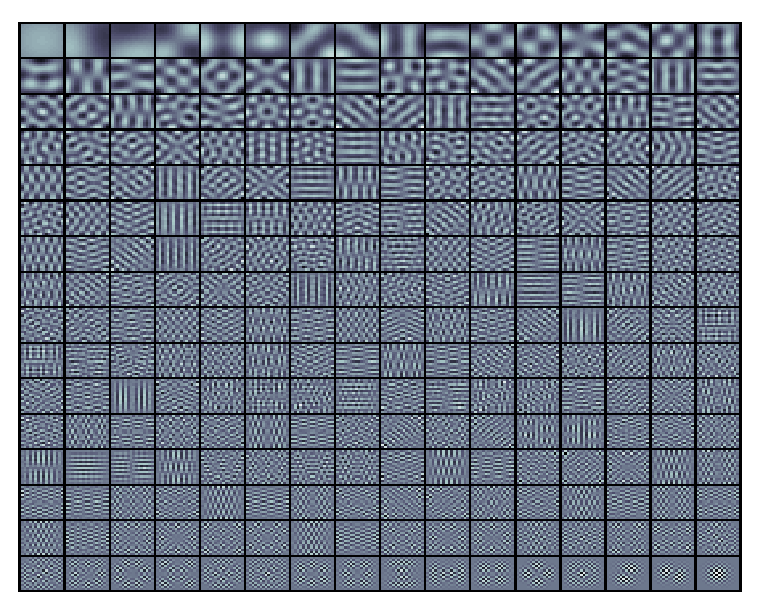
\includegraphics[width=0.45\textwidth]{./images/DL/DLstat/PCA_patchsize04.eps}
	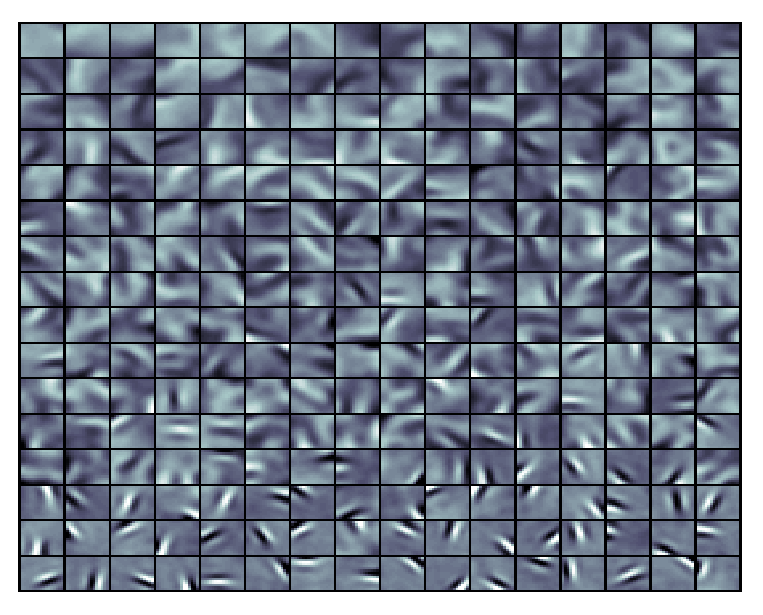
\includegraphics[width=0.45\textwidth]{./images/DL/DLstat/D_HR_lambda005.eps}
	\caption{\label{fig:PODvsDL} Dictionaries leaned by PCA and ODL from the set of HR patches of size $ \dimpsh = 16 \times 16 $. With ODL, only 256 atoms are chosen from 512 atoms.}
\end{figure}

Figure \ref{fig:PODvsDL} shows the adaptive dictionaries learned by PCA (left) and ODL (right) as ranked by their energy contents. The redundant dictionary by ODL has two times more atoms compared to PCA, which contains exactly $ \dimpsh = 16 \times 16 $ atoms as the dimension of the input patches. Only 256 over 512 atoms obtained by ODL are shown to be comparable with the PCA dictionary. The atoms are completely different in the two dictionaries. PCA dictionary has a sharp decline of variance content. Also, since the number of training patches is sufficiently large, the atoms look similar to discrete cosine transform (DCT) basis functions, which have modulated sine-wave patterns. The redundant dictionary from ODL contains more ``patterns'' for each level of scale, which is expected to be more adaptive to the data for sparse representation. 

Using a wavelet transform, there is no learning since the bases are predefined. The fields are decomposed into approximation and detail coefficients (horizontal, vertical and diagonal). The common Daubechies wavelet is used for its compact support and fast computation. The transform is performed on full fields. To test the sparsity effects, different thresholds are used. Detail coefficients larger than each threshold are retained while setting others to zeros, while approximation coefficients are kept unchanged. Inverse wavelet transform reconstructs the fields using these unchanged approximation and filtered detail coefficients. The sparsity is defined as the ratio of nonzero coefficients $ \dimtrunc $ (including both approximation and retained detail coefficients after filtering) and the dimension of the field $ \dimsh $. The NRMSE between reconstructed fields $ \hat{\z}_t $ and reference ones $ \z_t $ is estimated as in equation \ref{eq:NRMSE} to qualify the reconstruction for each level of sparsity $ (1- \dimtrunc/\dimsh )$.

With PCA, the dictionary $ \dict $ is learned from training patches $ \mathbf{P}_h $ extracted from all $ \left\lbrace \x_t \right\rbrace, t=1,...,\dimtl $. Its atoms  $ \left\lbrace \adicthigh{i} \right\rbrace $ are ranked by their variances $ \lambda_i $, i.e. $ \lambda_1 > \lambda_2 > ... > \lambda_{\dimsh} $. The dimensionality is reduced such that the retained information from only the first $ \dimtrunc $ principal components ($ \dimtrunc < \dimpsh $) is maximized. For a new field $ \z_t $, $ \mathbf{P}_h $ are extracted and projected onto the first $ \dimtrunc $ vectors:
\begin{equation}
	\adictco_i = \frac{\mathbf{P}_h \mydot  \adicthigh{i}}{\normtwo{\adicthigh{i}}} \:, i=1,2,...,\dimtrunc
	\label{eq:DL_efficiency3}	
\end{equation}
The filtered patches are estimated by combining the projected coefficients with the corresponding functions:
\begin{equation}
	\hat{\mathbf{P}}_h = \sum\limits_{i=1}^{\dimtrunc} {\adictco_i \adicthigh{i}}
	\label{eq:DL_efficiency4}
\end{equation}
Finally, the reconstructed field $ \hat{\z}_t $ is estimated by one-pixel overlapping as discussed in section \ref{subsec:patch_based_estimation}. The sparsity level is defined as $ 1-\dimtrunc/\dimpsh $, where the patch size at HR is $ \dimpsh = 16 \times 16 $. NRMSEs are estimated using equation \ref{eq:NRMSE}. 

KSVD and ODL learn $ \dict $ from $ \mathbf{P}_h $ \textit{a priori} with a high sparsity level ($ \lambda =0.2$, corresponding to about $ 15 $ non-zero coefficients). In the reconstruction step, all possible patches $ \mathbf{P}_h $ are extracted from each field $ \z_t $. The sparse code is estimated using LARS algorithm to solve:
\begin{equation}
	\dictco = \argmin_{\dictco} \left\lbrace \normtwo{\mathbf{P}_h - \dict \dictco_t} + \lambda \normone{\dictco} \right\rbrace
	\label{eq:DL_efficiency2}	
\end{equation}
The efficiency of the learned dictionary $ \dict $ is studied by varying $ \lambda $ in this step. For each $ \lambda $, $ \dictco $ is estimated and then used to re-estimate the patches $ \hat{\mathbf{P}}_h = \dict \dictco$ before reconstructing the global scene $ \hat{\z}_t $. Sparsity is measured as the average of $ 1- \normzero{\adictco_t}/\dimpsh $, where $ \adictco_t $ is the $ t- $th row of $ \dictco $. NRMSEs are estimated the same way as of wavelet transform or PCA.

\begin{figure}[t]
\centering
	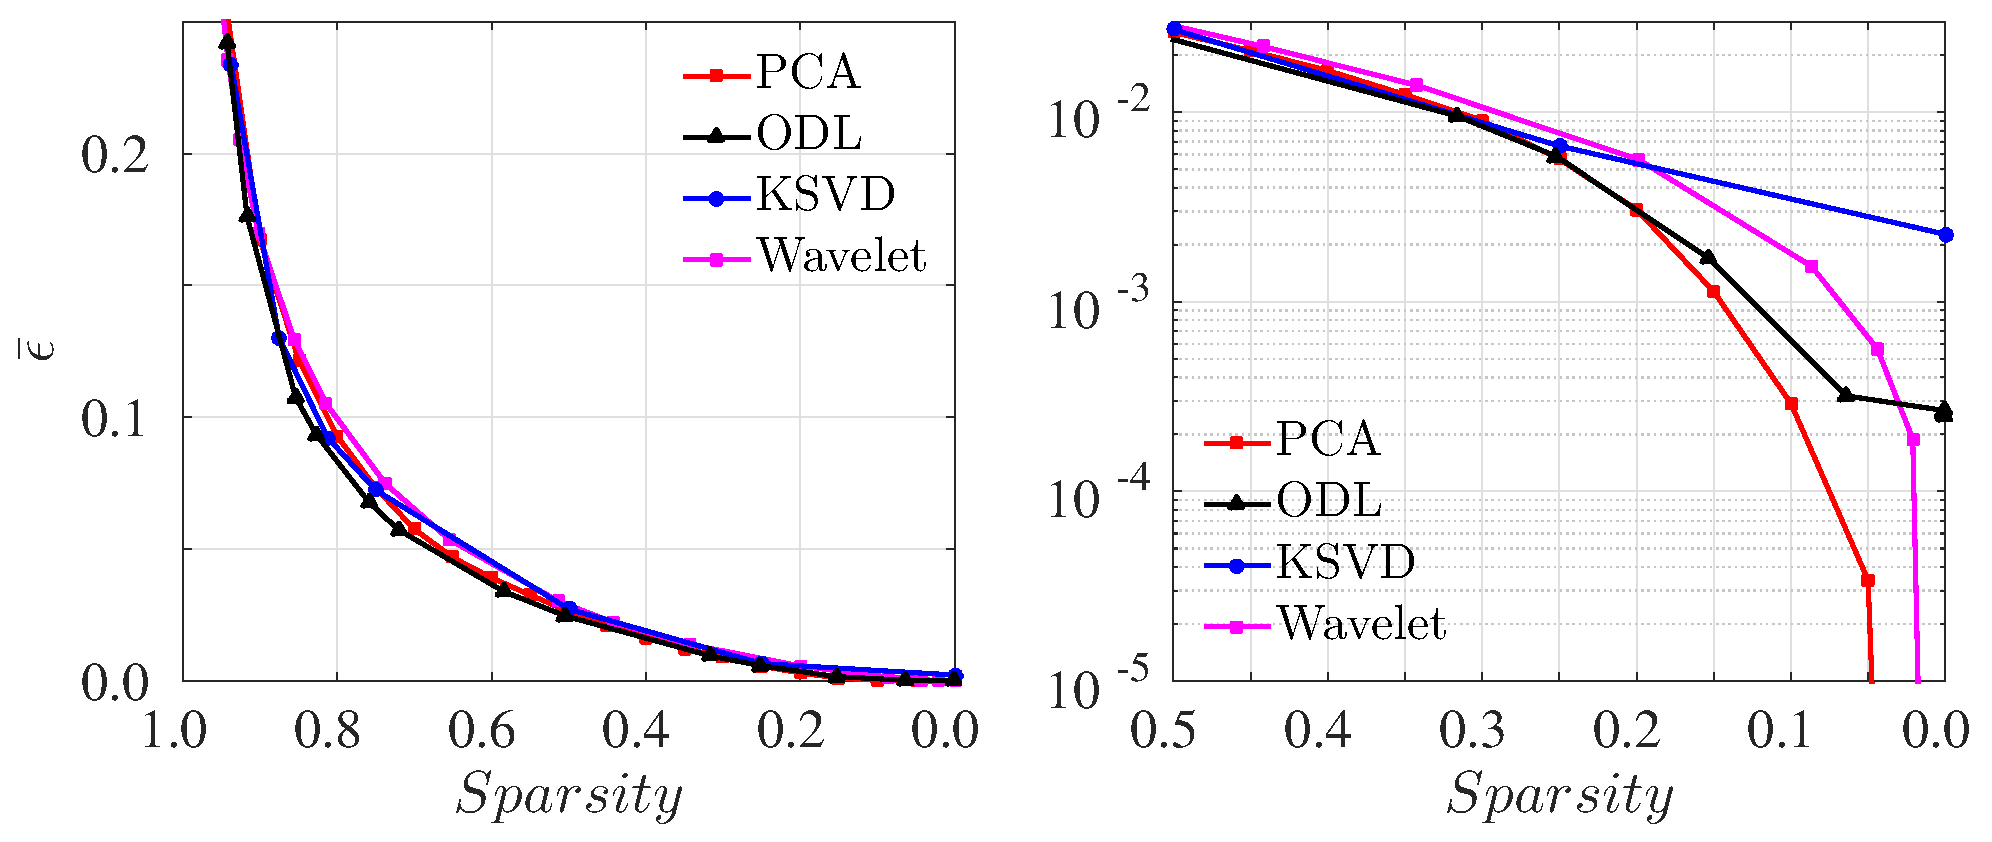
\includegraphics[width=\textwidth]{./images/DL/DLstat/Sparsity_vs_NRMSE_PCA_ODL_KSVD_WL_Dau_patchsize04.eps}
	\caption{\label{fig:Sparsity_vs_NRMSE} Sparsity vs error outside (left) and zoom in the region of low sparsity at semi-log scale (right) for different representations: wavelet (Daubechies), PCA, dictionary learning (ODL or KSVD). Wavelet transform is for the whole fields of size $ 96 \times 96$, while PCA and DL are for patches of size $ \dimpsh = 16 \times 16 $.}
\end{figure}

Figure \ref{fig:Sparsity_vs_NRMSE} shows the curves of NRMSE as functions of sparsity levels. These errors are estimated from five testing planes equally far from neighboring LTHS snapshots. All curves behave similarly as reducing the error when sparsity decreases. At high levels (larger than 0.5), there is a clear benefit of using DL. With the same number of non-zero coefficients, both ODL and KSVD give lower errors than PCA and wavelet transform. Few atoms from DL better represent the data than high variance principal components of PCA or predefined ones. Comparing the two DL methods, ODL is better than KSVD. When using more non-zero coefficients, errors by DL methods saturate at nonzero values. Since DL provides only an approximate solution. Wavelet transform and PCA give zero NRMSEs when using all coefficients because the transforms are exact.

The above comparisons demonstrate the advantages of representations using learned dictionaries over predefined ones. Comparing redundant and orthogonal representations, i.e. DL versus PCA, redundant dictionaries represent the fields more efficiently. They achieve the same level of error using less atoms. This suggests also that the sparsity and redundancy priors can be good candidates to help solving the ill-posed inverse problem of reconstructing HR fields from LR ones. Comparing the two common DL methods, ODL shows clear advantages both in term of efficient representation and computation effort and will be used in the rest of this chapter. 
 	
\subsection{Reconstruction of high resolution fields- subsampling cases}
To compare to other methods, LR fields are first subsampled from HR ones by a factor of $ 4 \times 4 $, i.e. $ \y_t = \Sub_s \z_t $, where $ \Sub_s: \R^\dimsh \mapsto \R^\dimsl $, $ \dimsh/\dimsl = 4 \times 4 $. Coupled LR and HR patches are extracted to train the dictionaries. Due to direct subsampling, the aliasing, which has not been addressed in previous works, will play an important role. This section investigates the ability of dictionary learning approaches to handle this aliasing problem.

\subsubsection*{Learning step}
\begin{figure}[t]
\centering
	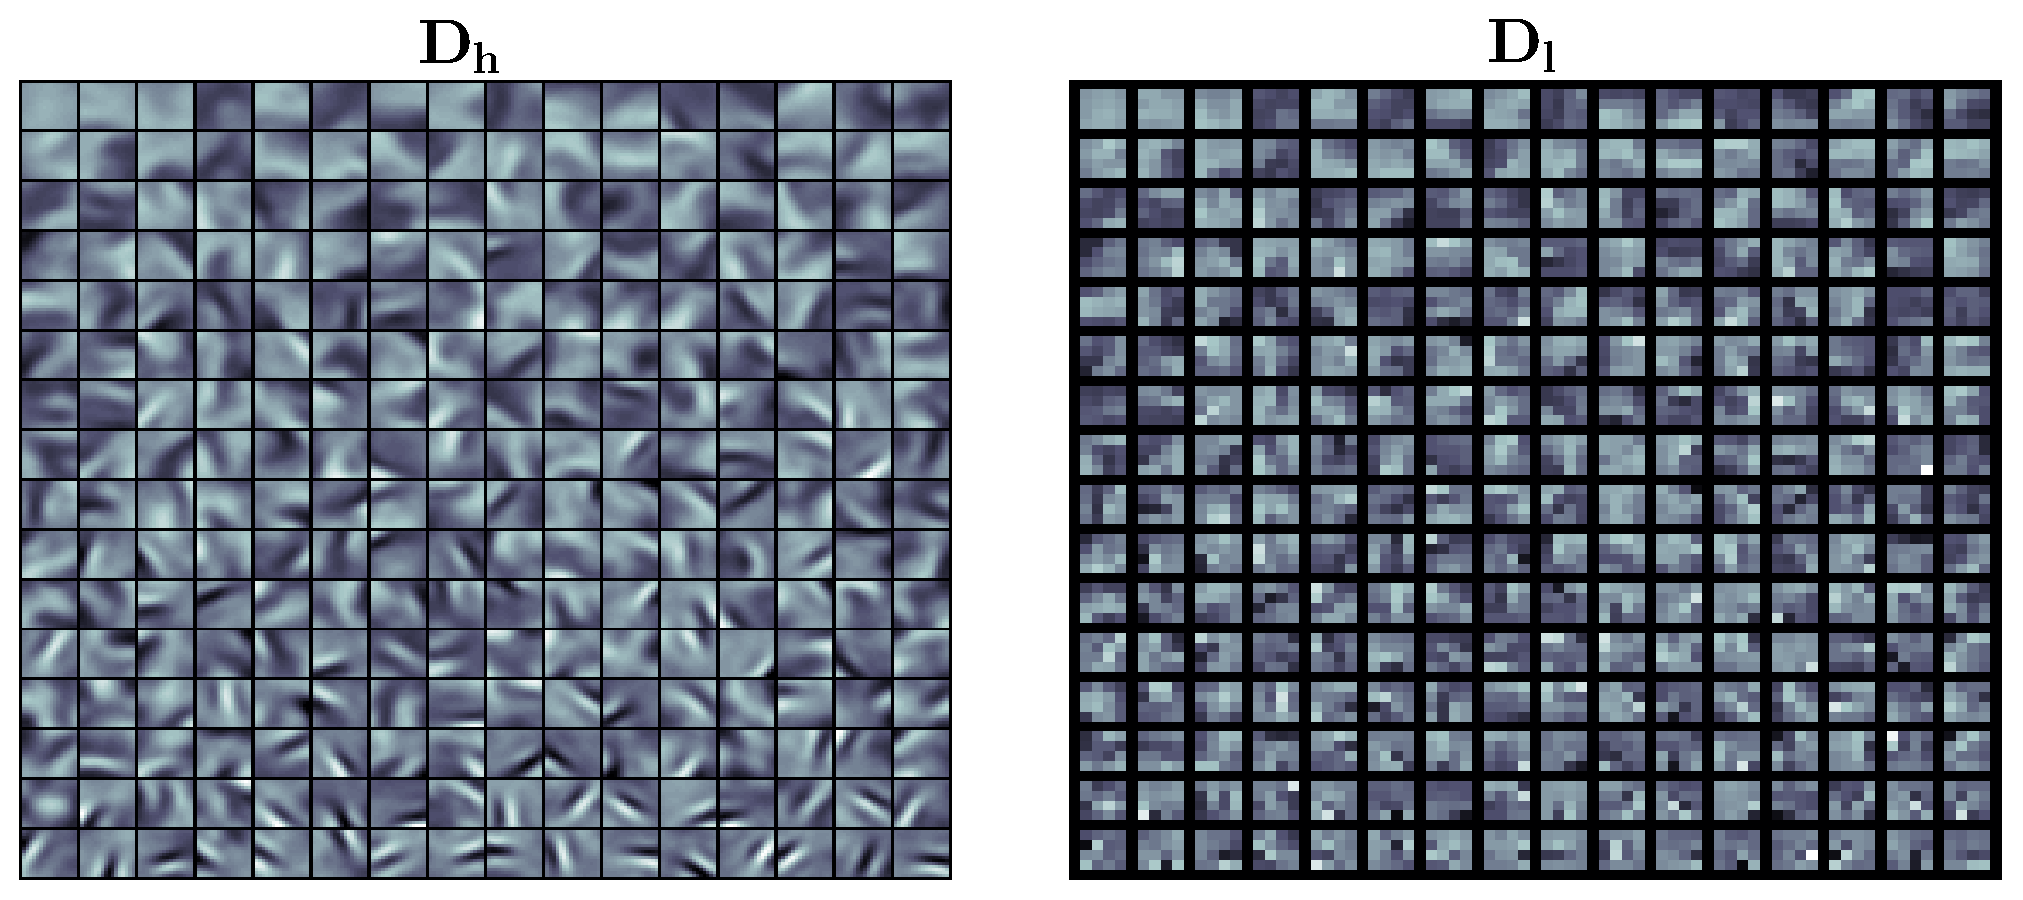
\includegraphics[width=\textwidth]{./images/DL/SR_sspacing04/subsampling/coupleddictionary_HRLR_lambda010.eps}
	\caption{\label{fig:D_HR_LR} Coupled dictionary of high and low resolution patches, with LR patches are of size $ 4\times 4 $, directly subsampled from their equivalent HR patches of size $ 16 \times 16 $. The regularization parameter $ \lambda $ for join learning are chosen such that about 16 non-zero coefficients are retained for reconstructing the joint patches of the training.}
\end{figure}

\begin{figure}[t]
\centering
	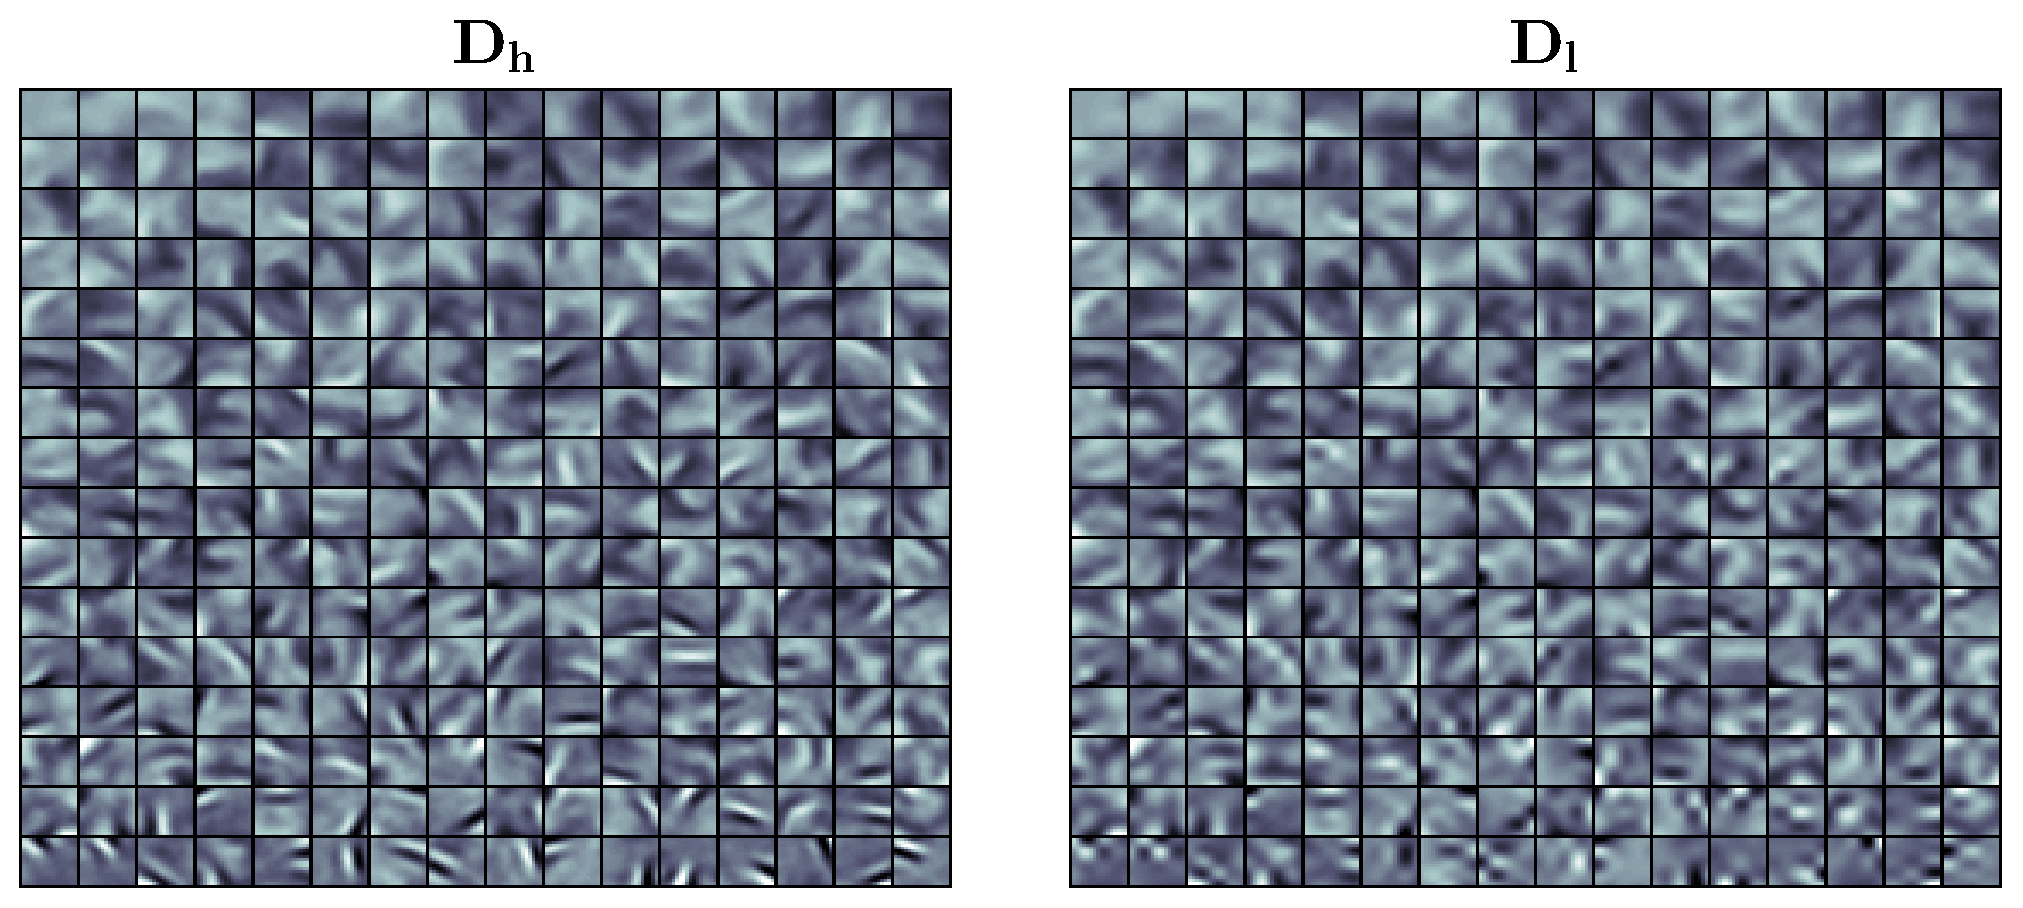
\includegraphics[width=\textwidth]{./images/DL/SR_sspacing04/subsampling/coupleddictionary_HRHRinterp_lambda010.eps}
	\caption{\label{fig:D_HR_HRinterp} Coupled dictionary of high and low resolution patches, where LR patches are of size $ 4\times 4 $, directly subsampled from their equivalent HR patches of size $ 16 \times 16 $. The regularization parameter $ \lambda $ for join learning are chosen such that about 16 non-zero coefficients are retained for reconstructing the joint patches of the training.}
\end{figure}

ODL \citep{mairal2010online} is used to learn a joint dictionary of HR and LR from the LTHS planes. The subsampling ratio in space is $ \dimsh/\dimsl = 4 \times 4 $, while the training samples are taken every $ \dimth/\dimtl = 6 $ snapshots in streamwise direction. From a total of $ 37 \times 16 $ training planes, small patches of size $ 4 \times 4 $ at LR are extracted via the extraction operator $ \extractlow{k} $, coupled with HR patches of size $ 16 \times 16 $ by $ \extracthigh{k} $. The choice of parameters is discussed in section \ref{subsec:DL_choice_params}.

Three approaches \textit{SR1}, \textit{SR2} and \textit{SR3} (table \ref{tab:DLapproaches}) are investigated. The interpolation step in \textit{SR2} plays only the role of transforming the field from LR to the same dimension as the HR one. The content should be rather the same, since the interpolation does not introduce any small-scale information. However, starting from the interpolated fields can bring the benefit of having a good large-scale information \textit{a priori}. The model will focus on small scales only. This approach have shown to be beneficial in many image processing problems.

Figure \ref{fig:D_HR_LR} shows dictionaries for HR and LR patches and figure \ref{fig:D_HR_HRinterp} shows dictionaries for HR and interpolated LR patches. In both figures, atoms are sorted according to their variances $ \normtwo{\adictco_i} $ when learning the dictionary (from the top-left). The most significant atoms contain mostly large scales, while less significant ones represent high-frequency contents. Coupled atoms show similar patterns. The relation between LR and HR patches are now encoded in the relation between LR and HR dictionaries. The assumption of coupled representations in this case also implies that LR atoms are approximately subsampled from the HR ones as shown in equation \ref{eq:DL_approach5}. 

\subsubsection*{Reconstruction step}
Having learned dictionaries $ \{\dicthigh,\dictlow \} $ at hand, from given $ \y^\ext $ different from the training data, the HR field $ \z^\ext $ is reconstructed by using algorithm \ref{algo_SR}. $ \y^\ext $ is also assumed to be directly subsampled from $ \z^\ext $ the same way as in the training data, i.e. $ \y^\ext = \Sub_s \z^\ext $. From $ \y^\ext $, all LR patches $ \mathbf{P}_l^\ext $ with one-pixel overlapping are extracted. The sparse code is estimated by solving the optimization problem in equation \ref{eq:algo_SR_4}. $ \dictco^\ext $ is then used to reconstruct HR patches as $ \hat{\mathbf{P}}_h^\ext = \dicthigh \dictco^\ext $ and put back into the global scene of $ \hat{\z}^\ext $. 

LR and HR patches of sizes $ \dimpsl = 4 \times 4 $ and $ \dimpsh = 16 \times 16$ respectively are extracted from all training planes. The sparse code $ \dictco^\ext $ is estimated from LR patches. Each row has at most $ \normzero{\dictco^\ext} = \dimpsl = 16 $ nonzero coefficients. It means that HR patches are reconstructed from maximum $ 16 $ atoms within $ \dicthigh $, a strong constraint on the reconstruction accuracy (see figure \ref{fig:Sparsity_vs_NRMSE}). The nature of the data also affects the accuracy in the sense how good is the Sparse-Land prior. Also, this constraint addresses the problem of designing more efficient representations of the data to reduce the error when using the same number of atoms. 

Using all three approaches presented in table \ref{tab:DLapproaches}, the models can reconstruct the fields in the same accuracy as the spline interpolation but not better. This is due to the severe situation where the presence of aliasing makes equation \ref{eq:DL_approach5} a very crude assumption. The subsampling of a small atoms brings a very strong aliasing effect that coupled dictionaries could not efficiently handle. The next section will study the capability of the present approach when the aliasing problem is absent from the LR data.

\subsection{Reconstruction of high resolution fields- the downsampling case}
\begin{figure}
	\centering
	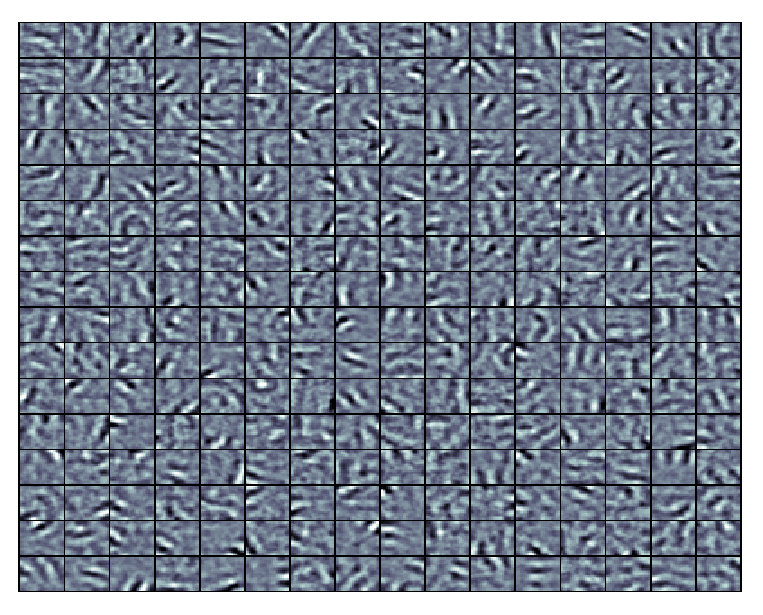
\includegraphics[width=0.6\textwidth]{./images/DL/SR_sspacing04/downsampling/dictionary_couplefeatures_patchesHR.eps}
	\caption{Dictionary of the residual between HR and interpolated LR.}
	\label{fig:SR_dictionary_residual}
\end{figure}

This section investigates the possibility of the current approach to estimate the HR fields given the LR ones in the case of downsampling, i.e. with anti-aliasing prefiltering:
\begin{equation}
\y_t = \Sub_s \LPF_s \z_t
\end{equation}
where $ \Sub_s $ and $ \LPF_s $ are the spatial subsampling and low pass filter respectively. Bicubic filter in Matlab built-in function \textit{imresize} is used for the prefiltering and interpolation step. It was shown also in section \ref{sec:chap3_theapproach} that the assumptions Sparse-Land model at HR also lead to the relation $ \mathbf{P}_\ell =  \Sub_s^\ext \LPF_s^\ext \mathbf{P}_h$ between LR and HR dictionaries. $ \Sub_s^\ext $ and $ \LPF_s^\ext $ are local versions of $ \Sub_s $ and $ \LPF_s $ applying to patches. 

We compare the three methods of coupled dictionary learning, the so-called \textit{SR1}, \textit{SR2} or \textit{SR3}, presented in table \ref{tab:DLapproaches}. To recall \textit{SR1} and \textit{SR2} couple either LR or interpolated LR patches with HR ones, while \textit{SR3} couples the residuals with the features of derivatives. The procedure follows the previous section of subsampled fields, with learning parameters in table \ref{tab:DLparams}. HR patches $ \mathbf{P}_h$ are extracted from LTHS fields and coupled with LR patches $ \mathbf{P}_\ell$. The dictionaries are trained \textit{offline} from $ \{\mathbf{P}_h, \mathbf{P}_\ell\}$, and used in \textit{online} reconstruction stage for all HTLS measurements to reconstruct HTHS fields. 

We use three quantities for comparisons: the average NRMSE between reconstructed and reference velocity fields estimated using equation \ref{eq:NRMSE}, the 2D energy spectra of the velocity fields and of the errors. These three quantities give a complete view to qualify different approaches. Only the most difficult planes, which are equally far from LTHS measurements, are used to estimate the errors. Error estimated using these planes will better represent the generalization capability of the approaches.

\begin{figure}
	\centering
	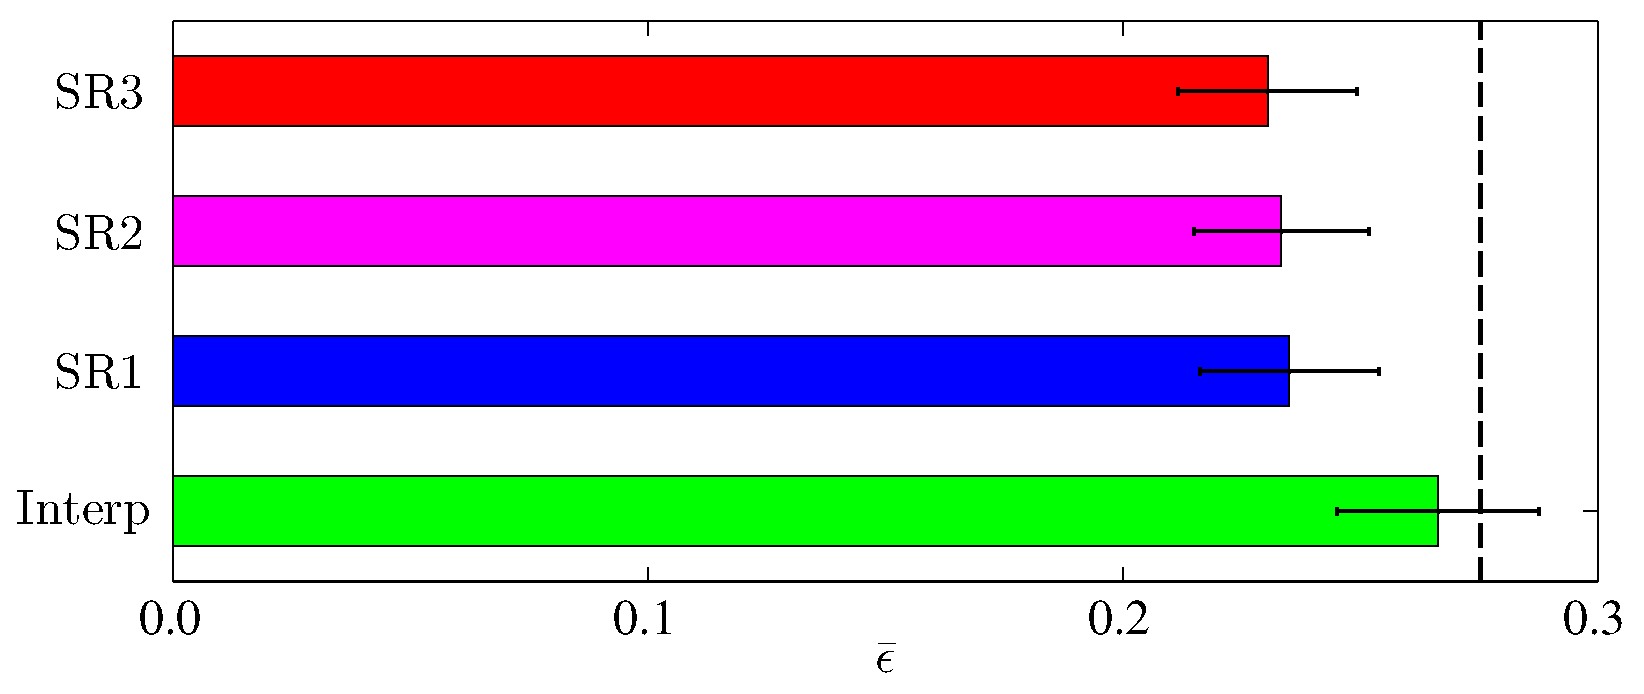
\includegraphics[width=0.9\textwidth]{./images/DL/SR_sspacing04/downsampling/NRMSE_compare_all_spacespacing_04.eps}
	\caption{Means and standard deviations of NRMSEs estimated between reference and reconstructed fields of all middle planes (at the center of blocks bounded by the two LTHS planes). The reconstructions are by spline interpolation and super-resolution using three different methods:: \textit{SR1}, \textit{SR2} and \textit{SR3} (see table \ref{tab:DLapproaches}). NRMSEs are $ 0.267 \pm 0.021 $, $ 0.235 \pm 0.019 $, $ 0.233 \pm 0.018 $ and $ 0.230 \pm 0.019 $ respectively. The NRSME of spline interpolation in the equivalent subsampling case is 0.276 (dashed black line).}
	\label{fig:NRMSE_compare_all_spacespacing_04}
\end{figure}

Figure \ref{fig:NRMSE_compare_all_spacespacing_04} shows the average NRMSEs of different reconstructions, either interpolation or reconstruction by coupled dictionaries using \textit{SR1}, \textit{SR2} or \textit{SR3} approaches. The three DL models reduce NRMSEs by $ 11.99 \% $, $ 12.73 \% $ and $ 13.86 \% $ respectively compared to the simple interpolation. \textit{SR3} gives the most accurate reconstructions by coupling the residuals, essentially contain only small scales, with derivatives of large-scale structures.

\begin{figure}
	\centering
	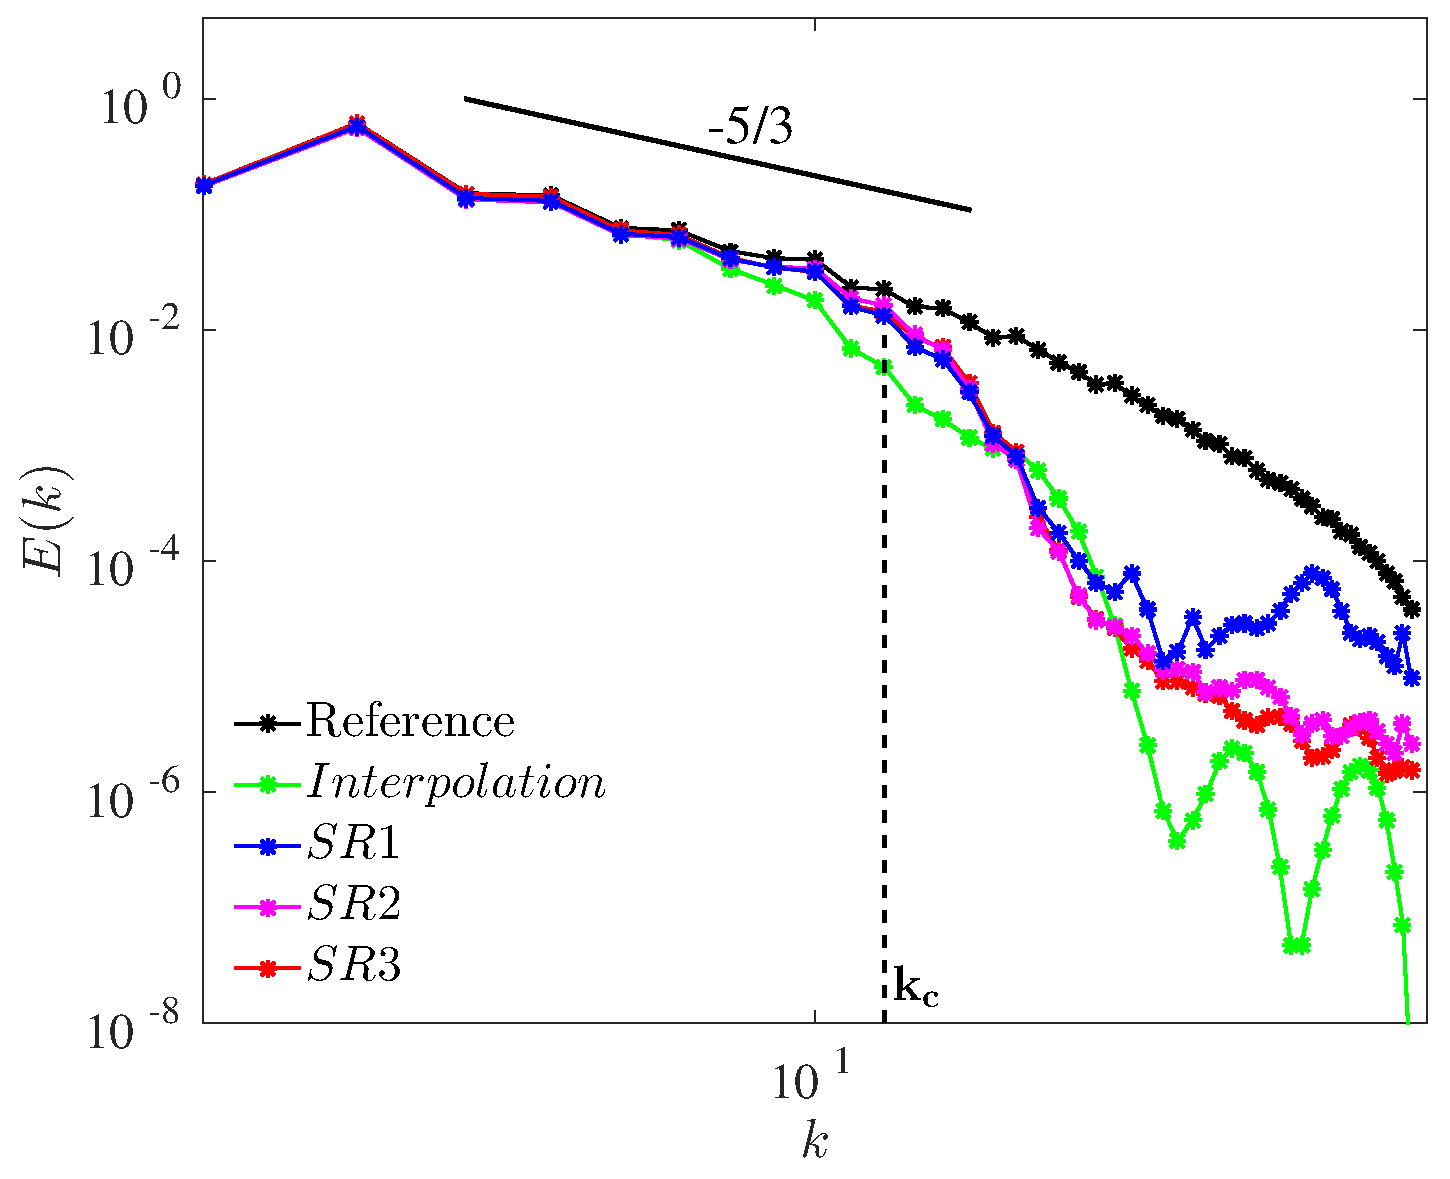
\includegraphics[width=0.75\textwidth]{./images/DL/SR_sspacing04/downsampling/spectra2d_spacespacing_04.eps}
	\caption{2D spectra of all planes used to computed the NRMSEs in figure \ref{fig:NRMSE_compare_all_spacespacing_04}, from reference, interpolation and SR by three different methods: \textit{SR1}, \textit{SR2} and \textit{SR3} (see table \ref{tab:DLapproaches}). For scales from $ 0.5k_c $ to $ 1.5 k_c$, energy losses of SR fields compared to reference ones is $ 24\% $, $ 22\% $ and $ 21\% $ respectively, while that of interpolation is $85 \% $.}
	\label{fig:spectra2d_spacespacing_04}
\end{figure}

To further understand the quality of the reconstructed fields at different scales, figure \ref{fig:spectra2d_spacespacing_04} shows the 2D spectra of reference fields and different reconstructed ones. All methods capture good large scales till about $ 0.5 k_c $, where $ k_c $ is the cutoff wave number defined by the subsampling ratio. The interpolation, starting from the downsampled fields with prefiltering step to avoid aliasing, loses already energy at large scales and capture almost no small scales. By coupling the dictionaries, the reconstructed fields recover the large-scale information with some small scales. If considering only the scales between $ 0.5k_c $ and $ 1.5k_c $, the energy loss of interpolated fields is $ 85\% $, while those are $ 24\% $, $ 22\% $ and $ 21\% $  for \textit{SR1}, \textit{SR2} and \textit{SR3} respectively. The benefit of SR is significant in this most interesting range of scales. Larger than $ 1.5k_c $, all reconstructions are not reliable. Smaller than $ 0.5 k_c $, spectra of all reconstructed fields are already very accurate. 

\begin{figure}
	\centering
	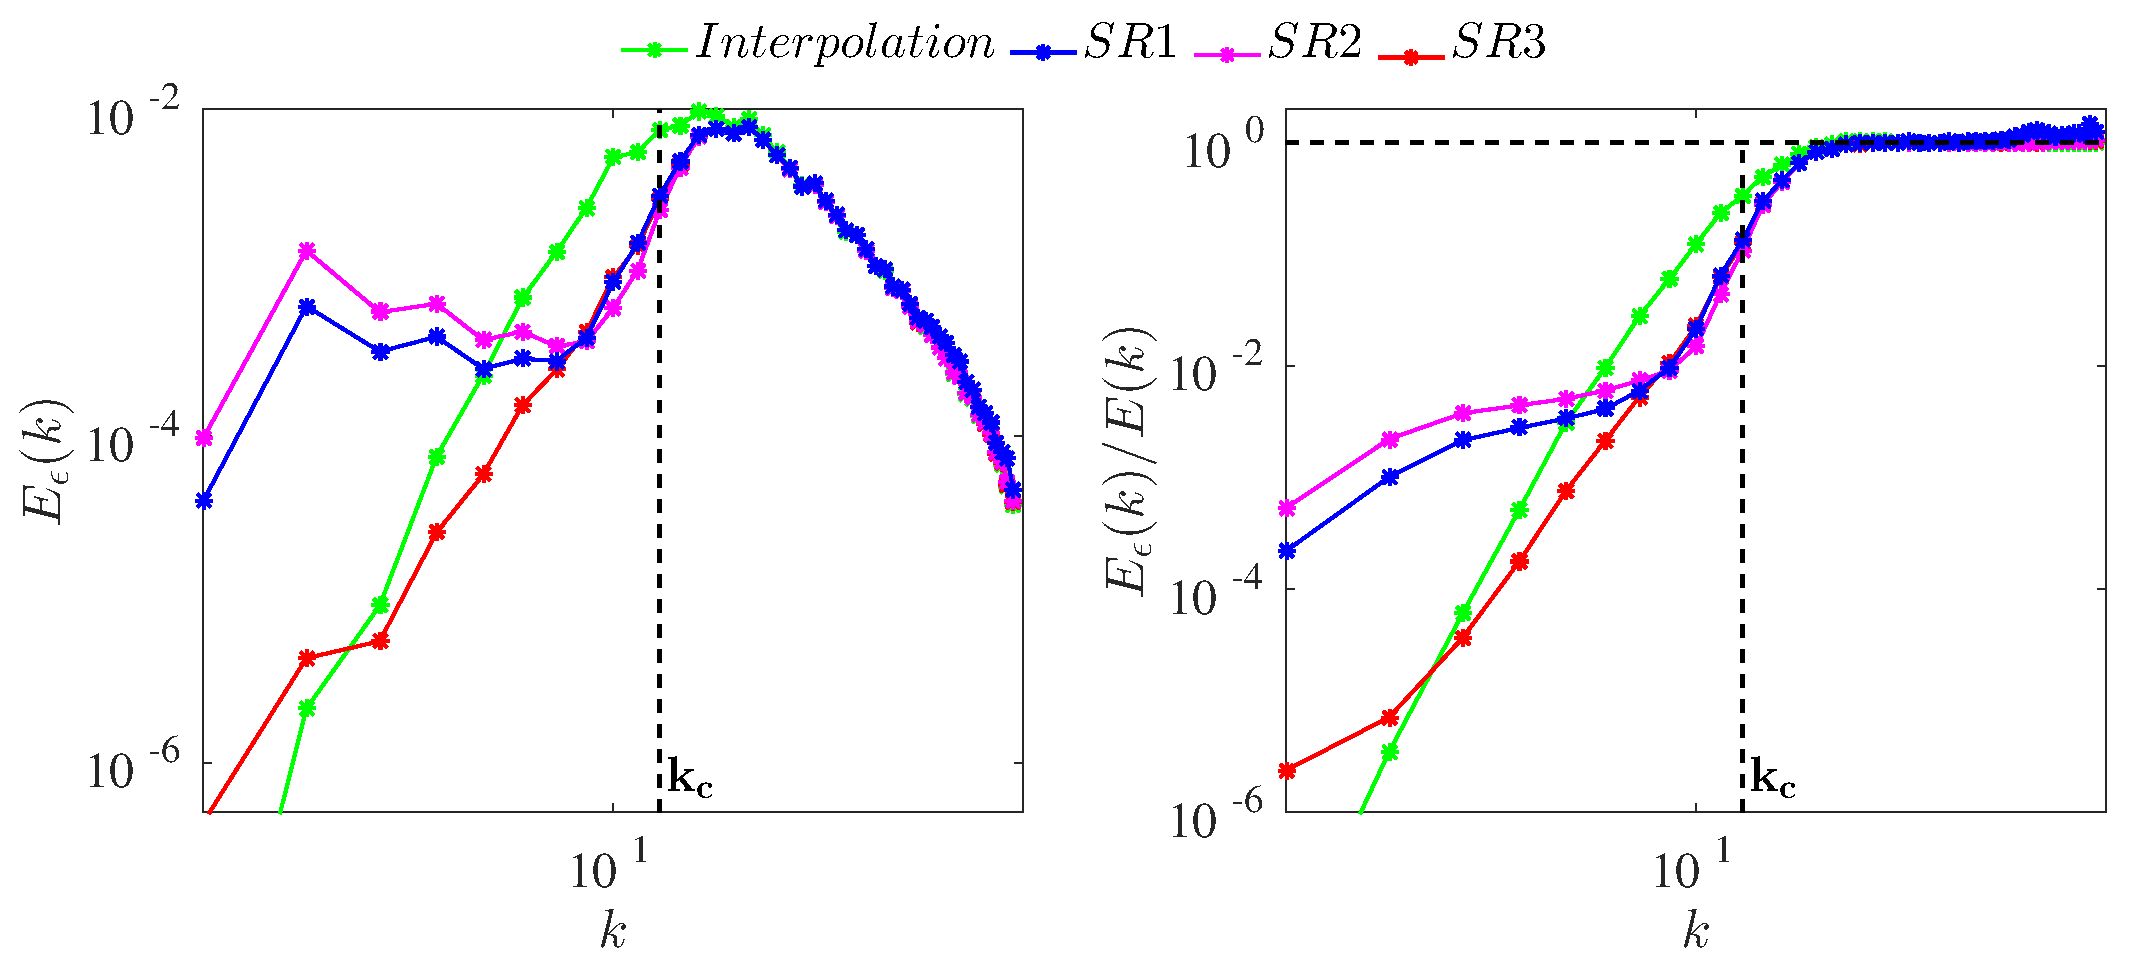
\includegraphics[width=\textwidth]{./images/DL/SR_sspacing04/downsampling/errspectra2d_nonnormalized_normalized_timespacing_06_spacespacing_04.eps}
	\caption{(Left) 2D spectra of errors, which are the different between the reference and reconstruction by interpolation and three different SR methods as described in \ref{sec:joint_learning_methods}. (Right) 2D spectra of errors normalized by the energy spectrum of the reference (the black curve in figure \ref{fig:spectra2d_spacespacing_04}).}
	\label{fig:errspectra2d_nonnormalized_normalized_timespacing_06_spacespacing_04}
\end{figure}

Figure \ref{fig:errspectra2d_nonnormalized_normalized_timespacing_06_spacespacing_04} (left) shows the spectra of the errors, which are the differences between the reference and reconstructed fields by all methods. Errors are very low at small wave numbers, reach a maximum around $ k_c $ and reduce at higher wave numbers. Integrals of these curves give the mean-square errors of each reconstruction method. To better qualify the error at each scale, the curves are normalized by the energy spectrum of the reference (the black curve in Figure \ref{fig:spectra2d_spacespacing_04}). The normalized spectra of errors are interpreted as the percentage of error at each scale. The interpolation gives very small relative errors at large scales, but grow rapidly near $ k_c $. Error spectra of all SR methods collapse at $ 0.5k_c $ and reach a maximum of $ 100 \% $ error at around $ 1.5k_c $. Smaller than $ 0.5k_c $, \textit{SR1} and \textit{SR2} gives slightly higher errors compared to \textit{SR3}. \textit{SR3} is more accurate since it starts from the interpolated large scales, while those information are re-estimated by \textit{SR1} and \textit{SR2}. Also, \textit{SR3} focuses more on the missing information of small scales by using derivatives as features and following the patterns of larger ones. 

From the above comparisons, coupled dictionary approaches demonstrate clear benefits compared to the simple interpolation, with errors reduced by about $ 15\% $. From the energy spectra or spectra of errors, the benefits mostly come from the range of scales between $ 0.5k_c $ and $ 1.5k_c $, where $ k_c $ is the cutoff defined by the grid of LR measurements. The loss of energy in this range is reduced from $ 80\% $ with interpolation to $ 20\% $ by DL approaches. The spectra of the errors also show that most of benefits come from this range of scales, before reaching $ 100\% $ at around $ 1.5k_c $.

\section{Concluding remarks}
This chapter has discussed the possibilities of applying dictionary learning, a successful approach in the field of signal and image processing, to turbulence studies. The method finds a representation for the data by generalizing principal component analysis to sparse representation in a redundant dictionary. \textit{Redundancy} means that the number of atoms can be larger than the dimension of input vectors, ignoring the orthogonality constraint of PCA. This implies the \textit{sparsity}, i.e. the representation is composed by a linear combination of only a few atoms. These properties make the learned dictionary a more adaptive representation of the data. Sparsity can also play the role of a prior about the system when solving the inverse problem of HR field reconstruction. 

To investigate the efficiency of DL in representing the data, the learned dictionaries by this approach have been compared against PCA and predefined wavelet dictionaries. Reconstruction errors as functions of sparsity, i.e. the number of atoms used, are shown as the measure of efficiency. Adaptive dictionaries show some superiority compared to the predefined ones. The benefits are mainly from the high sparsity levels, when less than half the number of coefficients are non-zero. 

DL is then used to reconstruct HR velocity fields from LR measurements. The approach is called \textit{coupled dictionary learning}, inspired from the single image super-resolution application \citet{yang2010image,zeyde2012single}. By learning coupled representations of LR and HR fields from the data, a nonlinear relation is established and generalized to perform the reconstruction task. With the same idea, different preprocessing techniques are tested. The coupling can be between HR and LR fields or their interpolation. Another approach focuses more on the small-scale information by coupling the small scales with the derivatives of interpolated fields. 

The first attempt is for the configuration where LR fields are directly subsampled from HR ones without any anti-aliasing prefiltering step. This is \textit{a priori} not a favorable case due to the presence of aliasing terms. However, it is worth studying since this setup mimics what would happen in a real experiment. It is interesting also to see how well learned dictionaries can handle aliasing. Results show that DL is inoperative to recover some small scales on top of the interpolated large-scale information. 

To understand whether the failure comes from the approach or from the aliasing, another case is investigated where LR fields are downsampled from the HR ones with a prefiltering step. The same approach with  identical parameters is used. Results show significant improvements of reconstruction accuracy, with about $ 15 \% $ reduction of NRMSEs compared to interpolation. Spectral analyses also show that most benefits are at the frequency range of $ 0.5 k_c$ to $ 1.5k_c $, where $ k_c $ is the cutoff wave number corresponding to the downsampling ratio. In term of energy, simple interpolation loses $ 85 \% $ in this range scales, while this loss is reduced to about $ 20 \% $ with DL approaches.

The above results demonstrate the capability and limitations of DL approaches in solving the reconstruction problem in turbulence. The corresponding prior, which is the duality between sparsity and redundancy, is robust. The first attempt has not succeeded to reconstruct HR fields from direct subsampled LR ones due to the aliasing problem. This attempt addresses also the question on designing a good sensing system or post-processing techniques to deal with aliasing terms if exist.

This chapter has presented a similar configuration as regression models to learn the mapping function between large and small scales. However, the learning is localized thanks to the patch-wise approach. This property of dictionary learning approach can be beneficial when applying to other configurations where the training and testing samples are of different scenes. For example, the training HR fields could be a small region of the whole field, while LR one can be larger. In such case, dictionary approach is the only candidate among all methods presented in this thesis. 


